\documentclass[12pt,dvipdfmx]{jreport}
\usepackage{comment}
\usepackage{./sty/eclepsf}
\usepackage{tascmac}
\usepackage{tabularx}
\usepackage{listliketab}
\usepackage[longnamesfirst]{natbib}
\usepackage{graphics}
\usepackage{graphicx}
\usepackage{booktabs}
\usepackage{color}
\usepackage[table,xcdraw]{xcolor}
\usepackage{subfigure}
\usepackage{alltt}
\usepackage{here}
\usepackage{afterpage}
\usepackage{./sty/ncodeline}
%\usepackage[dvipdfmx, colorlinks, breaklinks,%
\usepackage[dvipdfmx, breaklinks,%
bookmarks=true, bookmarksnumbered=true,%
bookmarkstype=toc, bookmarksopen=true,bookmarksopenlevel=3,%
pdftitle={Dynamic advertising method of Explicit Address Mapping in IPv6 single stack network.},%
]{hyperref}
\usepackage{bookmark}

\AtBeginDvi{\special{pdf:tounicode EUC-UCS2}}

\usepackage{fancyhdr}

\usepackage{./sty/doxygenorig}

\usepackage{indentfirst}
\usepackage{url}
\usepackage{listings,./sty/jlisting}

\def\lstlistingname{プログラム}

\lstset{
  basicstyle={\ttfamily},
  identifierstyle={\small},
  commentstyle={\smallitshape},
  keywordstyle={\small\bfseries},
  ndkeywordstyle={\small},
  stringstyle={\small\ttfamily},
  frame={tb},
  breaklines=true,
  columns=[l]{fullflexible},
  numbers=left,
  xrightmargin=0zw,
  xleftmargin=3zw,
  numberstyle={\scriptsize},
  stepnumber=1,
  numbersep=1zw,
  lineskip=-0.5ex
}

\usepackage{amssymb}
%\usepackage{supertabular,multirow}

\usepackage{array}
\newcolumntype{M}[1]{>{\centering\arraybackslash}m{#1}}

% A4  size: 297mm*210mm %1pt = 0.35mm
\setlength{\topmargin}{-3.4mm} % 10pt 25.4mm - 3.4mm = 22mm
\setlength{\oddsidemargin}{-0.4mm} % 25.4mm - 0.4mm = 25mm
\setlength{\evensidemargin}{-0.4mm} % 25.4mm - 0.4mm = 25mm
\setlength{\textheight}{231mm} % 660pt % original is 225.75mm 645pt
\setlength{\textwidth}{160mm} % 457pt

\renewcommand{\topfraction}{.99}
\renewcommand{\textfraction}{.0}
\renewcommand{\floatpagefraction}{.99}
\renewcommand{\bibname}{参考文献}


\pagestyle{fancy}
\lhead[]{}

\makeatletter
\def\chaptermark#1{\markboth {\ifnum \c@secnumdepth>\m@ne
\@chapapp\ \thechapter \@chappos\ \fi #1}{}}
\makeatother

% タイトル
\def\title{IPv6シングルスタックネットワークにおける\\ダイナミックなアドレス変換テーブル広告手法}
% 英語タイトル
\def\etitle{Dynamic advertising method of \\ Explicit Address Mapping in IPv6 single stack network.}
% 著者(日本語)
\def\author{豊田 安信}
% 著者(英語)
\def\eauthor{Yasunobu Toyota}
% 学部・研究科
\def\dept{慶應義塾大学大学院 政策・メディア研究科}
% 学部・研究科(英語)
\def\edept{Keio University Graduate School of Media and Governance}

\begin{document}

\pagenumbering{roman}
\begin{titlepage}
  \begin{center}
    \begin{large}
      修士論文   2019年度(令和元年度)\\
      \vspace{24pt}
      \title
      \end{large}
  \end{center}
  \vspace{40em}
  \begin{flushright}
    \large \dept\\
    \author
  \end{flushright}
\end{titlepage}

\thispagestyle{empty}


修士論文要旨 - 2019年度 (令和元年度)
\begin{center}
\begin{large}
\begin{tabular}{|M{0.97\linewidth}|}
    \hline
      \title \\
    \hline
\end{tabular}
\end{large}
\end{center}

2019年現在,ライブ映像配信のようなリアルタイムなサービスに対するニーズが高まっていることや,災害・地政学的リスクの回避を目的として,IDC(Internet Data Center)・コンテンツ事業者を中心にコンテンツ配信基盤拠点を各地域に分散する取り組みが活発である.

一方で2020年頃には各地域レジストリからIPv4アドレスの新規割当が行えなくなることが予想されているほか,2016年にIAB(Internet Architecture Board)によりインターネット標準はIPv6に最適化した標準策定を行う方針が確認されており,IPv4を前提とした長期的なネットワーク運用は限界を迎えていると言える.事業者がビジネスを拡大するためには,IPv4アドレスを極力使用しないIPv6シングルスタックネットワークの活用が不可欠になっている.

しかしながら2019年現在においてもIPv4によるトラフィックは依然としてインターネット全体の大きな割合を占めていることから,IPv6シングルスタックネットワークでありながらIPv4によるサービスを継続して提供可能なネットワーク設計が必要である.

IPv6シングルスタックネットワークにおいてIPv4によるサービス提供を行う方法として,"SIIT-DC"と呼ばれるネットワークデザインがインターネット標準化されている.SIIT-DCではBR(Border Relay)と呼ばれる変換機構をIPv4インターネットとIDC内のIPv6ネットワークの境界点に設置し,アドレス変換テーブル(EAMT:Eplicit Address Mapping Table)を参照してプロトコル変換を行うことで,IPv6サーバでのIPv4サービス提供を可能にする.しかしながらSIIT-DCではEAMTの動的な交換方法についての定義がなされておらず,EAMTが一貫しない場合にサービスの冗長性を維持出来ない点や,IPv4でサービス提供を行なうサーバの構成変更が行われた場合に個別の運用が必要になる点が課題に挙げられる.

本研究ではBGP(Border Gateway Protocol)を利用したアドレス変換テーブルの広告・更新技術を提案する.これにより,SIIT-DCの課題であったサービスの冗長性や変更追従性に対して柔軟に対応するIPv6シングルスタックネットワークの構築が可能になる.

本手法を評価するために,新たにBGPによるアドレス変換テーブル制御機構を実装したソフトウェアルータを用いた評価実験用ネットワークを構築した.本評価環境を用いて概念検証実験を行い,EAMTの一貫性の維持や変更追従性及びスケーラビリティの面で,本手法が効果的に作用することが証明された.

~ \\

キーワード:\\
\underline{1. データセンターネットワーク},
\underline{3. ネットワークオペレーション},
\underline{4. IPv6移行技術}
\begin{flushright}
\dept \\
\author
\end{flushright}

\thispagestyle{plain}
\clearpage

Abstract of Bachelor's Thesis - Academic Year 2020
\begin{center}
\begin{large}
\begin{tabular}{|M{0.97\linewidth}|}
    \hline
      \etitle \\
    \hline
\end{tabular}
\end{large}
\end{center}

In recent years,load balancers have been shifting from hardware appliances to software. In this way, data centers have solved the physical space and economic cost problems. These high-speed software load balancers are designed to improve packet processing performance by using high-speed data plane technology that utilizes kernel bypass packet processing frameworks, etc.

However, these high-speed data plane technologies cannot utilize existing control plane APIs, and developers are spending more resources on control plane development than on data plane.

In this study, we designed and implemented shadowLB, a mechanism that transparently accelerates only the data plane while reusing the existing control plane functions. We have shown that shadowLB can achieve X times performance in tail latency while using the ipvs API, which is the de facto standard for existing control planes.


% The transition from the IPv4 Internet to the IPv6 Internet is gaining momentum at present. Many ISPs (Internet Service Providers) have already completed the environment improvement of the IPv6 access network by operating in IPv4/IPv6 dual-stack network. Client devices such as PCs and smartphones have been required to use IPv6. In the client devices represented by PC and smartphone, the utilization of IPv6 becomes very popular.

% In this situation, the correspondence to the IPv6 access of companies that provide content services via the Internet lags behind. It is expected that the new allocation of IPv4 addresses will not be possible from each regional registry. In addition, the IAB (Internet Architecture Board) confirmed its policy in 2016 that Internet standards should be optimized for IPv6. Therefore, IDC operation based on IPv4 is not continuous. In other words, the utilization of IPv6 single stack network that does not use IPv4 addresses as much as possible is indispensable for IDC content providers to expand their business.

% However, it is necessary to design a network that can continuously provide the service by IPv4 even though it is the IPv6 single stack network because IPv4 traffic still accounts for the majority of all of the Internet traffic. 

% The "SIIT-DC" network design has been standardized as a way to provide IPv4 services in an IPv6 single-stack network. In SIIT-DC, equipment which called BR (Border Relay) is connected between IPv4 Internet and IPv6 IDC network translate IPv4 and IPv6 mutually by referring to Explicit Address Mapping Table (EAMT) in order to enable IPv4 service provision in IPv6 server. 

% Nevertheless, the dynamic advertisement method of EAMT does not define at SIIT-DC standards. This causes a lack of EAMT consistency. Because of it, SIIT-DC has two problems such as lack of redundancy in the multihoming network and enlargement of the operation load when a server is added or removed. "Dynamic EAMT" mechanism which manipulates EAMT of BR dynamically is required.

% In this paper, we propose an advertisement and update method of EAMT utilizing BGP (Border Gateway Protocol). BGP is a popular dynamic routing protocol and can maintain the consistency of routing information in response to changes in the state of BGP peers.
% The proposed method can construct the IPv6 single stack network flexibly corresponding to redundancy and reducing operational load which is the problem of SIIT-DC. This paper also propose a more scalable Dynamic EAMT mechanism using multilayered route reflectors.

% I implemented a software BR whose EAMT manipulated by BGP and a proof-of-concept network for evaluation experiments. 
% The evaluation experiments show that the proposed method can dynamically control the EAMT of 30 BRs inconsistent from the information of up to 600 IPv4 servers by using a 1 layer route reflector topology. In addition, by adopting the multilayer route reflector topology, it was clarified to correspond to the larger-scale network.

% This research proved that this method worked effectively in EAMT problems mentioned above, and is expected to improve the quality of IPv4 service provision in IPv6 single stack networks of future IDC network design.

~\\ 

Keywords : \\
\underline{1. Data center network},
\underline{2. Network operation},
\underline{3. IPv6 transition mechanism}
\begin{flushright}
\edept \\
\eauthor
\end{flushright}

\thispagestyle{plain}
\clearpage

\tableofcontents\thispagestyle{plain} %目次
\clearpage
\listoffigures\thispagestyle{plain} %図目次
\clearpage
\listoftables\thispagestyle{plain} %表目次
\clearpage

\pagenumbering{arabic}
\chapter{序論}
\label{introduction}
本章では本研究の背景とモチベーション,および全体の構成について記述する.

\section{IPv6シングルスタックネットワークに求められる役割}
\label{introduction:background}

\subsection{IDCネットワークを取り巻く環境}
\subsubsection{IDC市場の広がり}
% 単純にIDC事業が伸びていることを言う.


近年,ライブ映像配信のようなリアルタイムなサービスに対するニーズが年々高まっている.例えばCisco社の調査\cite{index2017global}によれば,2022年には全てのアプリケーショントラフィックのうちインターネットビデオが有する割合が82%を超え,そのうち17%がライブ映像配信が占めると予想されている.
リアルタイムな高品質サービスを提供するためには,ユーザーの地理的に近いサービス拠点から配信を行うことが有効であるため,今後IDC・コンテンツ事業者が各地域拠点を介したコンテンツ配信基盤を活用するしていくことが予想される.

% 災害リスクから拠点を増やしたい話
一方で,インフラストラクチャに対する災害や地政学的リスクの軽減は,コンテンツ事業者の継続的な事業の成長のためには避けては通れない課題である\cite{alonso2001business}.
2011年に発生した東日本大震災以降,国内のIDC事業者やコンテンツ事業者を中心に,関東大都市圏に集中していたサービス拠点への依存性を解消するために,東京圏以外の各地域にサービス拠点を分散する取り組みが活発だ\cite{JANOG44_robust}.大阪・名古屋の他の都市圏のIDCは2019年現在満床状態が続いているほか,他の地方拠点都市も含めたIDC建設も並行して行われている. 

特に近年ではVXLANやSRv6のような新しいネットワーク仮想化技術の標準化も進み,サービス拠点のマルチテナンシーと柔軟性を両立するネットワークデザインの障壁が低くなってきているため,今後より多くのIDC・コンテンツ事業者のサービス拠点の拡大が続くと想定できる.


\subsubsection{IPv4アドレスの枯渇}
\label{introduction:background:ipv4_problems}
2019年現在,IANA\footnote{Internet Assigned Numbers Authority.インターネットに利用される様々な資源を一元的に管理する組織.\url{https://www.iana.org/}}が保有するIPv4アドレスプールは既に枯渇しており\cite{IANA_allocation},各RIR\footnote{Regional Internet Registry.}からも2021年頃までには新規割当が行えなくなることが予想されている\cite{potaroo_IPv4}.

\begin{figure}
	\centering
	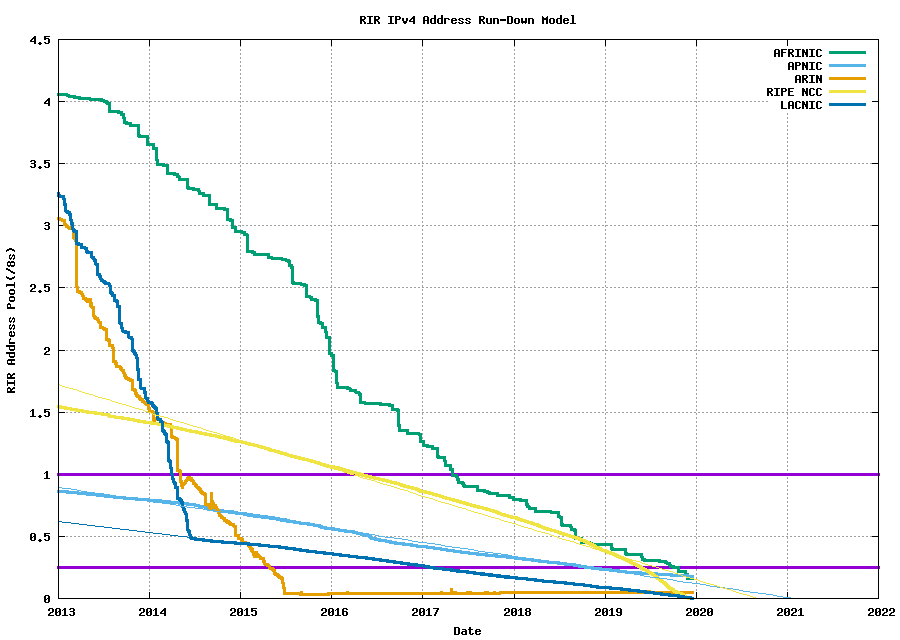
\includegraphics[width=12cm]{img/plotend.png}
	\caption{Projection of consumption of Remaining RIR Address Pools. \url{potaroo.net}より引用\cite{potaroo_IPv4}}
	\label{fig:potaroo_IPv4}
\end{figure}
    
一方で近年は民間事業者間アドレス取引も盛んに行われている.一般に新規にIPv4アドレスの割当を受けるためにはこのような民間取引市場を利用する方法が考えられるが,1アドレスあたりの単価は年々上昇傾向にあり\cite{howard2013internet},新規にIPv4ネットワークを構築するためのコストは日々上昇していくことが考えられる.


\subsubsection{IPv6への移行}
\label{introduction:background:ipv6_transition}
1998年に初めてのIPv6標準仕様が策定されて以降\cite{RFC2460},IPv6インターネットとIPv4インターネットの独立した二つのインターネットが並行して存在する状態が2019年現在まで続いている.

一方でインターネット技術はIPv6を前提とした設計が行われる段階を迎えている.2016年にはIAB\footnote{Internet Architecture Board. \url{https://www.iab.org/}}により,"IAB Statement on IPv6"が発表され,インターネット標準はIPv6に最適化標準策定を行う方針が確認されている\cite{IAB_statement}.例えば既にSRv6のような新しい標準はIPv6の拡張ヘッダーを利用した技術として策定が進められており,IPv4を前提とした長期的なネットワーク運用は限界を迎えていると言える.

\subsubsection{IPv4/IPv6デュアルスタックネットワークの問題}
\label{introduction:background:dualstack_problems}
IPv6プロトコルの導入に主に用いられていた手法としてIPv4/IPv6デュアルスタックネットワークが挙げられる\cite{durand2001deploying}.IPv4/IPv6デュアルスタックネットワークとは,IPv4ネットワークとIPv6ネットワークを同一機器群上に並行して運用する手法であり,企業・一般家庭向けアクセスネットワークを中心にIPv4/IPv6デュアルスタック環境の整備が進んでいる.

一方でコンテンツ事業者が運用するIDCでは以下の主な3つの理由からデュアルスタック環境の導入はデメリットが大きい.

\begin{itemize}
    \item \textbf{IPv4アドレスの継続的調達が困難} \\
    先に述べたように,IPv4アドレスをサービスの成長にあわせて継続的に調達していくことは困難である.民間市場の市況に調達コストが左右されるため長期的な見通しが立てにくい.
    \item \textbf{オペレーションコストの肥大化}\\
デュアルスタック環境では2つの異なるIPプロトコルを同時に運用する必要があるため、シングルスタック環境と比べて運用コストの上昇が見込まれる\cite{北口善明2017クライアント}.
    \item \textbf{ネットワーク機器の性能要件の上昇}\\
デュアルスタック環境では,シングルスタック環境よりも多くの経路をネットワーク機器が保持しなければならないため,より高性能な機器を導入する必要がある.
\end{itemize}



\subsection{IPv6シングルスタックネットワーク}
\label{introduction:background:IPv6-single-stack-network}
IDC事業者・コンテンツ事業者がビジネスを健全に拡大するためには,IPv6ネットワークのみで機器間を接続したIPv6シングルスタックネットワークの利用が不可欠である.

IDCのIPv6シングルスタックネットワークには以下のような働きが期待される.


\subsubsection{IPv4サービスの提供}
\label{introduction:background:IPv6-single-stack-network:ipv4-service}
Google社が定常的に行っている調査\cite{Google_IPv6_statistics}によれば,2019年12月現在全世界のインターネットトラフィックの7割程度をIPv4トラフィックが依然として占めている.
将来的にはIPv6によるアクセスの割合が徐々に大きくなることが予想されるが,今後しばらくはIPv4クライアントに対してもIPv6クライアントと同等にサービス提供を行っていくことが望ましい.

コンテンツ事業者のIPv6シングルスタックネットワークにおいても,何らかの手段を用いてIPv4サービスを継続して提供する機構を備える必要がある.

\subsubsection{シングルスタック運用によるOPEX/CAPEXの削減}
第\ref{introduction:background:dualstack_problems}項で述べたように,IPv4/IPv6デュアルスタックネットワークではオペレーションコストの肥大化が問題視されていた.
IPv6シングルスタックネットワークではIPv4ネットワークを廃止することが出来るため,OPEX\footnote{Operating expense. 運用に掛かる継続的なコスト.}とCAPEX\footnote{Capital expenditure. 設備配備に掛かる初期投資コスト.}の軽減が期待される.
またIPv6アドレスはIPv4アドレスと比較して広大なアドレススペースを有するため,アドレススペースに依存しない柔軟なネットワーク設計が可能になる.

\subsubsection{IPv4/IPv6デュアルスタックネットワークと同等以上の性能}
IPv6により提供されるサービスはもちろんのこと,IPv4によるサービスにおいてもIPv4/IPv6デュアルスタックネットワークと同等の耐障害性・サービス品質・サービス容量が保証されることが望ましい.

とりわけネイティブなIPv4ネットワーク以外の手段を用いて提供されるIPv4サービスの性能の担保が運用課題になると予想される.




\section{本研究のモチベーションと取り組み}

第\ref{introduction:background:IPv6-single-stack-network}項で述べたようなIPv6シングルスタックネットワークに求められる要件のうち,IPv4サービスの提供における冗長性や構成変更への追従性の向上を促す手法の確立を目指す.

本研究ではIPv6シングルスタックネットワークにおけるIPv4サービスの提供手法のうち,アーキテクチャがシンプルで広範な利活用が期待されるSIIT-DC\cite{RFC7755}に着目した.
SIIT-DCとはIPv6ネットワークとIPv4ネットワークの各境界部に,BR\footnote{Border Relay. IP/ICMP変換アルゴリズム\cite{RFC7915}を実装したIPv4/IPv6トランスレーション機器.}を配備することにより,IPv6ネットワークのみに属するホストで仮想的にIPv4サービスを提供するネットワーク設計を定めたインターネット標準である.SIIT-DCにおいて各BRは静的に定義されたアドレス変換テーブルを利用してネットワークプロトコル変換を行うため,BRを複数配備する場合における一貫性の確保や冗長性,IDC内の構成変更に対する追従性の面で課題があった.

本研究では動的経路アルゴリズムの一つであるBGP\cite{RFC4271}を利用したメッセージングによるアドレス変換テーブルの動的な広告手法を提案する.
エミュレータを利用した概念実証実験により,本提案手法がこれらの課題に対して効果的に作用することが証明された.



\section{本論文の構成}

本論文の構成を以下に示す.

~第\ref{related}章では,IPv6シングルスタックネットワークにおけるIPv4サービス提供手法に関してそれぞれの特徴や利点を紹介し比較する.

~第\ref{issue}章では,IPv4/IPv6プロトコル変換を利用したIPv4サービス提供手法の一つであるSIIT-DCのアーキテクチャと,解決すべき課題について述べる.

~第\ref{consideration}章では,SIIT-DCの課題を解決するために考えられる手法を比較・検討する.

~第\ref{proposal}章では,本研究において提案するダイナミックなアドレス変換テーブル広告手法の要件と構成について記述する.またメッセージングプロトコルとして採用したBGPの技術的利点について述べる.

~第\ref{implementation}章では,本提案手法のBGPメッセージペイロードの設計と第\ref{evaluation}章でも評価実験に用いるPoCの具体的な実装について紹介する.

~第\ref{evaluation}章では,第\ref{issue}章で述べた課題に対して,本提案手法が有用であることを検証するための実証実験の概要及び具体的なシナリオについて述べ,結果を考察する.

~第\ref{conclusion}章では,本研究のまとめと今後のロードマップについて検討する.

%%% Local Variables:
%%% mode: japanese-latex
%%% TeX-master: "../thesis"
%%% End:

\chapter{IPv6シングルスタックネットワークでのIPv4サービス提供手法}
\label{related}
本章ではIPv6シングルスタックネットワークでのIPv4サービス提供手法を比較し,検討する.


\section{概要}
\label{related:abstract}


第\ref{introduction:background:IPv6-single-stack-network}項で述べたように,コンテンツ事業者が運用するIPv6シングルスタックネットワークの重要な役割の一つに,IPv4クライアントに対するサービス提供がある.

関連して,アクセスネットワーク網ではIPv6シングルスタックネットワーク上でIPv4によるインターネット接続をクライアントエッジに提供する手法はIPv4aaS(IPv4 as a Service)と呼称し,様々な手法が検討されている\cite{RFC8585}.

一方でコンテンツ事業者が運用するネットワークでのIPv4サービス提供においては次項で示す要件を満たす必要があるため,必ずしもアクセスネットワークでのIPv4aaSと同様の方法が適切であるとは限らない.

\subsection{IPv4サービス提供機構に求められる要件}
\label{related:abstract:requirements}
IPv6シングルスタックネットワークにおいて,サービス提供サーバがIPv4サービスを提供するためには,以下のような機能を有する必要がある.

\subsubsection{IPv4クライアントからのアクセス}
IPv6クライアントと同様に,IPv4クライアントに対しても透過的にサービスを提供する機構を備える必要がある.
一般的なサーバクライアントモデルを想定した場合,インターネット上のIPv4クライアントからサービス提供サーバに能動的に接続するためには,FQDN\footnote{Fully Qualified Domain Name. 完全就職ドメイン名}もしくはIPv4アドレスを指定出来る必要がある.


\subsubsection{スケーラビリティ}
近年のコンテンツ事業者のネットワークでは,サービスのニーズに合わせて柔軟にスケールアウト\footnote{水平スケール.同等性能の機器を増減させることでサービス容量を拡大・縮小可能なモデル.}可能な設計であることが重要視されている\cite{5550998}.同様にIPv4サービスの提供手法に関しても,事業者のIPv4サービス規模の変化にあわせて柔軟に拡大・縮小可能なアーキテクチャが求められる.

例えば,第\ref{introduction:background:IPv6-single-stack-network:ipv4-service}項でも述べたように,将来的にIPv4クライアントの占める割合がIPv6クライアントに相対して低下していった場合に,既設のIPv6ネットワークへの影響を最小限にしつつ,IPv4サービス提供機構を縮小可能であることが望ましい.


\subsubsection{IPv4ネットワークへの非依存性}
第\ref{introduction:background:IPv6-single-stack-network}項で述べたように,IPv6シングルスタックネットワークのメリットを最大限に活かすためにはIPv4サービスを提供する場合においてもIPv4ネットワーク及びアドレスに極力依存しないことが望ましい.



\section{IPv4サービス提供手法の分類}
\label{related:compare}
想定されるIPv4サービス提供機構をその技術的差異や狙いを基に以下の3つの手法に分類した.

\subsection{L7リバースプロキシ}

\begin{figure}[h]
    \begin{center}
      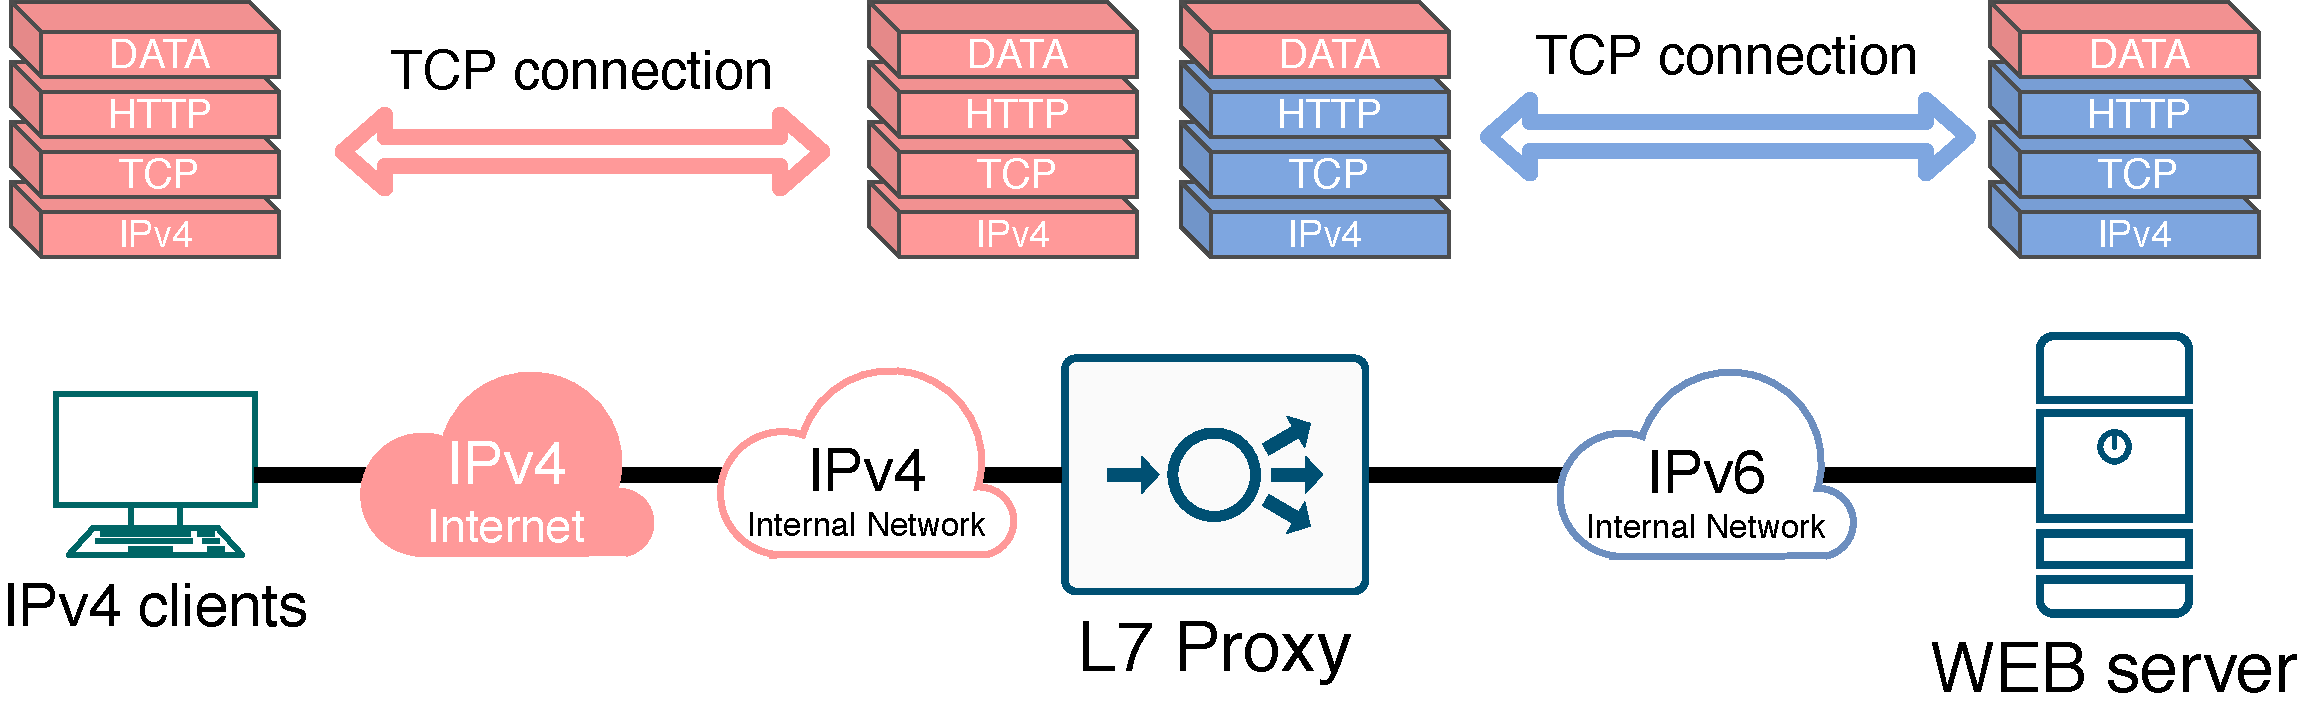
\includegraphics[width=15cm,pagebox=cropbox,clip]{img/L7_proxy_model.pdf}
    \end{center}
    \caption{L7リバースプロキシによるIPv4サービス提供}
    \label{fig:L7_proxy_model}
\end{figure}


L7リバースプロキシとは,クライアントからの接続をプロキシサーバがアプリケーション層レベルで終端し,プロキシサーバがクライアントに代わってサーバと接続する機構である\cite{Gilly2011}.図\ref{fig:L7_proxy_model}に本手法の構成を簡便に示す.プロキシサーバを用いる構成は,主にWEBサーバへのHTTP接続を負荷分散するための手法として広く採用されている.

IPv6シングルスタックネットワークにおいてIPv4サービスを提供するためには,IPv4インターネットとの接続点からプロキシサーバまでの間にIPv4ネットワークを配備する必要がある.

IPv4・IPv6間のプロトコル仕様の差を考慮する必要が無いため互換性に留意する必要が無い点や,MTU\footnote{ここでは一つのパケットに収容可能なデータ量を指す.}を減らさずにアプリケーショントラフィックを伝送可能である点が利点として挙げられる.

一方でアプリケーションレイヤーでのコネクション終端やそのステート管理を行う必要があるため,プロキシサーバに負荷が掛かるため高性能な機器の導入が必要になる.

またスケールアウトを可能にするためにL4LB(Layer4 Load Balancer)\footnote{トランスポート層レベルでの負荷分散を行う機器.}と組み合わせたマルチステージのアーキテクチャを利用する手法が近年主流であるが\cite{Facebook_LB, Google_LB},この手法を採用するためには,L4LB及びプロキシサーバにまでIPv4ネットワークを配備する必要があり,\ref{related:abstract:requirements}項で述べた要件に合致せず,IPv6シングルスタックネットワークのメリットを損なうことになる.



\subsection{IPv4/IPv6トンネリング}
\begin{figure}[h]
    \begin{center}
      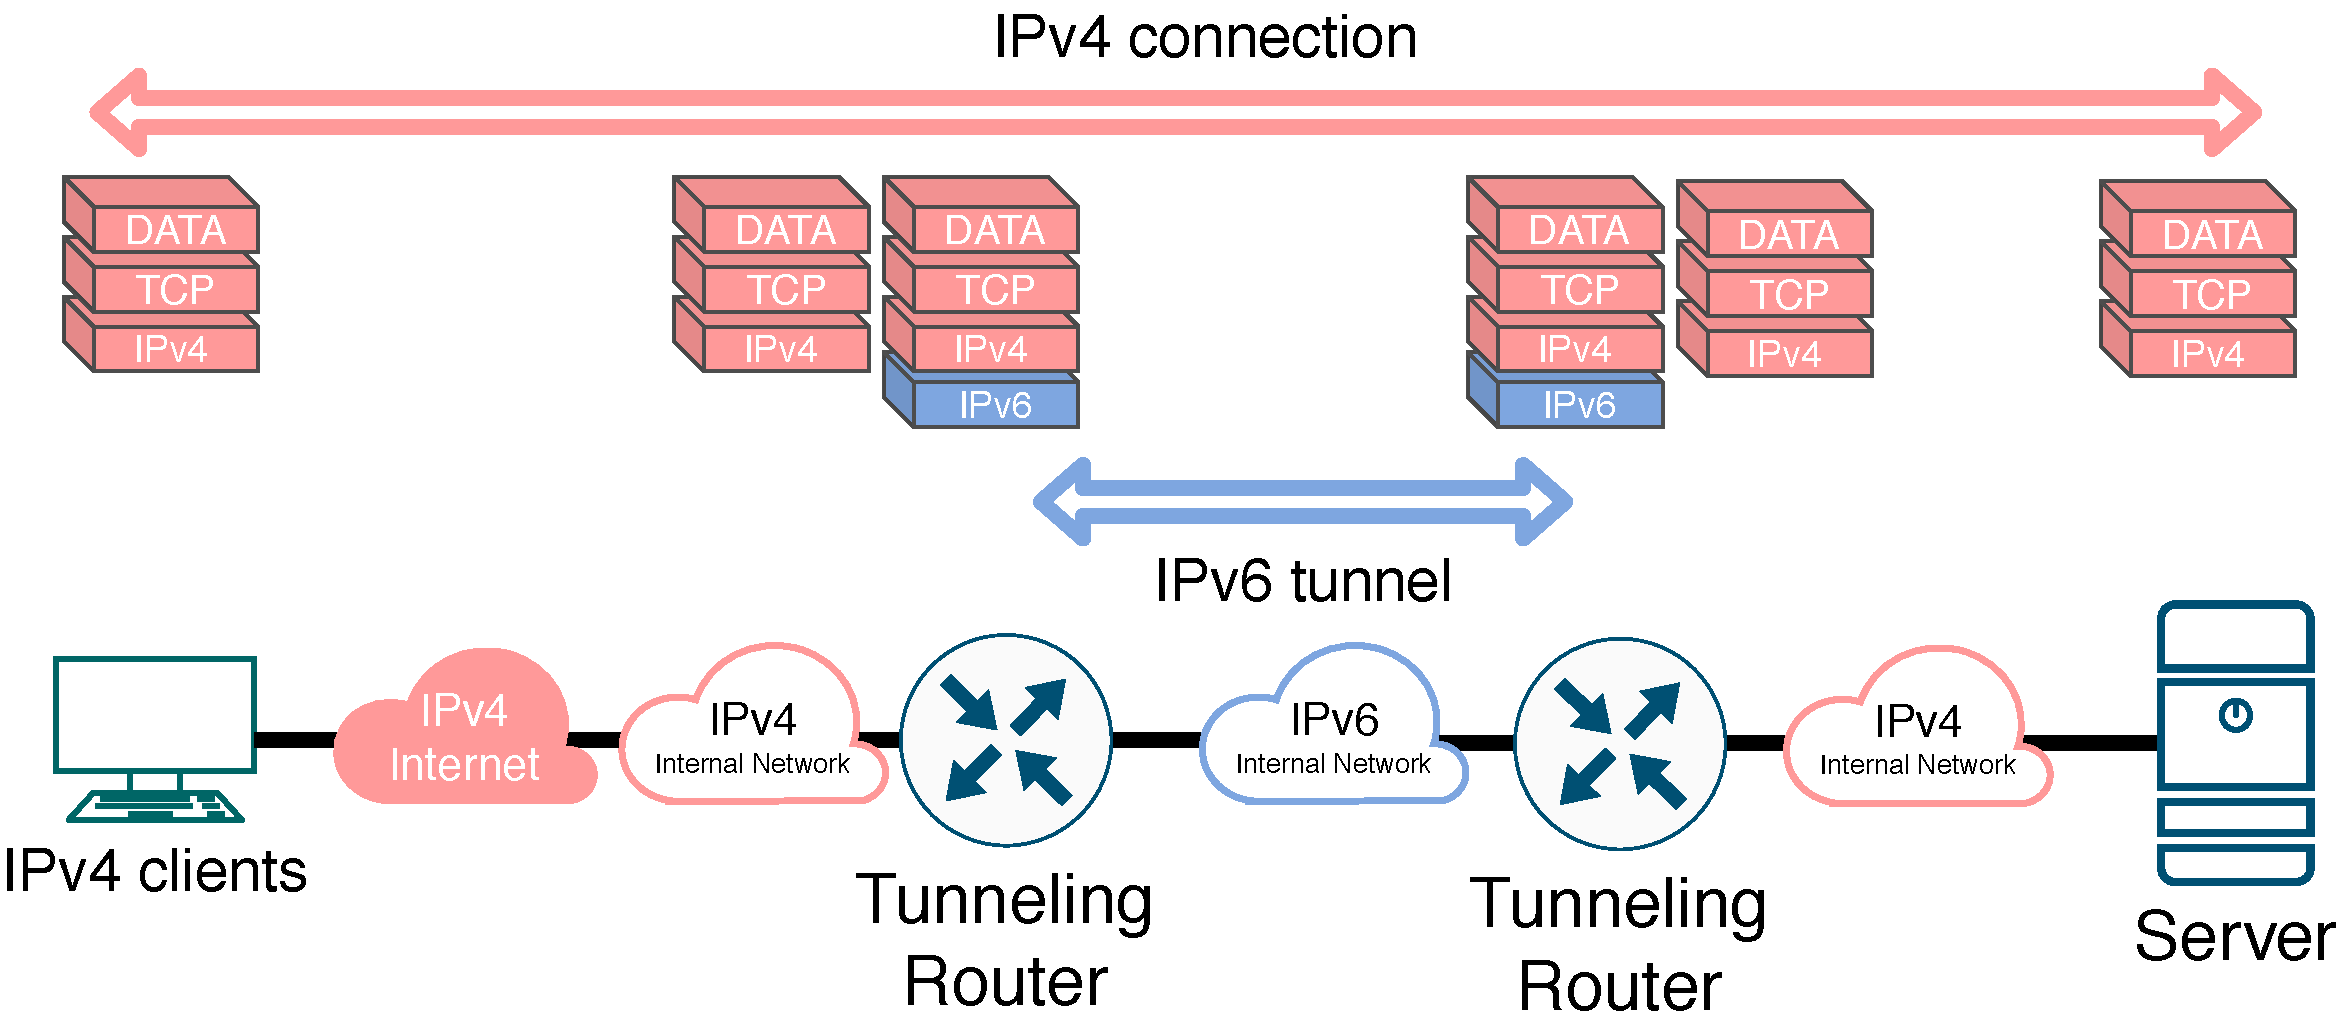
\includegraphics[width=15cm,pagebox=cropbox,clip]{img/Tunneling_model.pdf}
    \end{center}
    \caption{IPv4/IPv6トンネリングによるIPv4サービス提供}
    \label{fig:tunneling_model}
\end{figure}

IPv4/IPv6トンネリングとは,IPv4パケットをIPv6パケットによってカプセリングすることでIPv6ネットワークを通過させる手法である.IPv4トラフィックを透過的に利用することが出来るため,アクセスネットワークでのIPv4aaS実現手法として広く利用されている\cite{RFC8585}.図\ref{fig:tunneling_model}に本提供手法の構成を簡便に示す.

IPv6シングルスタックにおけるIPv4サービス提供手法としては,IPv4クライアントから到達したパケットをトンネルルータによって一度IPv6パケットでカプセリングし,IDC内のIPv6シングルスタックネットワークを通過させ,IPv4サービス提供サーバ上もしくはその直前で再びでカプセリングを解くことで,IPv4提供サーバまでネイティブなIPv4トラフィックを通過させる運用が考えらえる.
IPv4パケットをそのままサーバまで届けることが出来るため,多種多様なアプリケーションでのサービス提供が可能である.

しかしながら,トンネルルータとIPv4サービスサーバ間にIPv4ネットワークを配備しなければならず,ToR(Top of rack switch)\footnote{ここではサーバのL2終端を行うイーサネットスイッチを指す.}及びサーバではIPv4/IPV6デュアルスタック運用が必要になるため,第\ref{related:abstract:requirements}項で上げた要件である「IPv4ネットワークへの非依存性」を満たすことが出来ない.また,トンネルプロトコルの多く\cite{6799698}は基本的に1:1もしくは1:Nの接続が基本となるため,スケールアウトさせることが困難である.



\subsection{IPv4/IPv6トランスレーション}
\label{related:compare:translation}
\begin{figure}[h]
    \begin{center}
      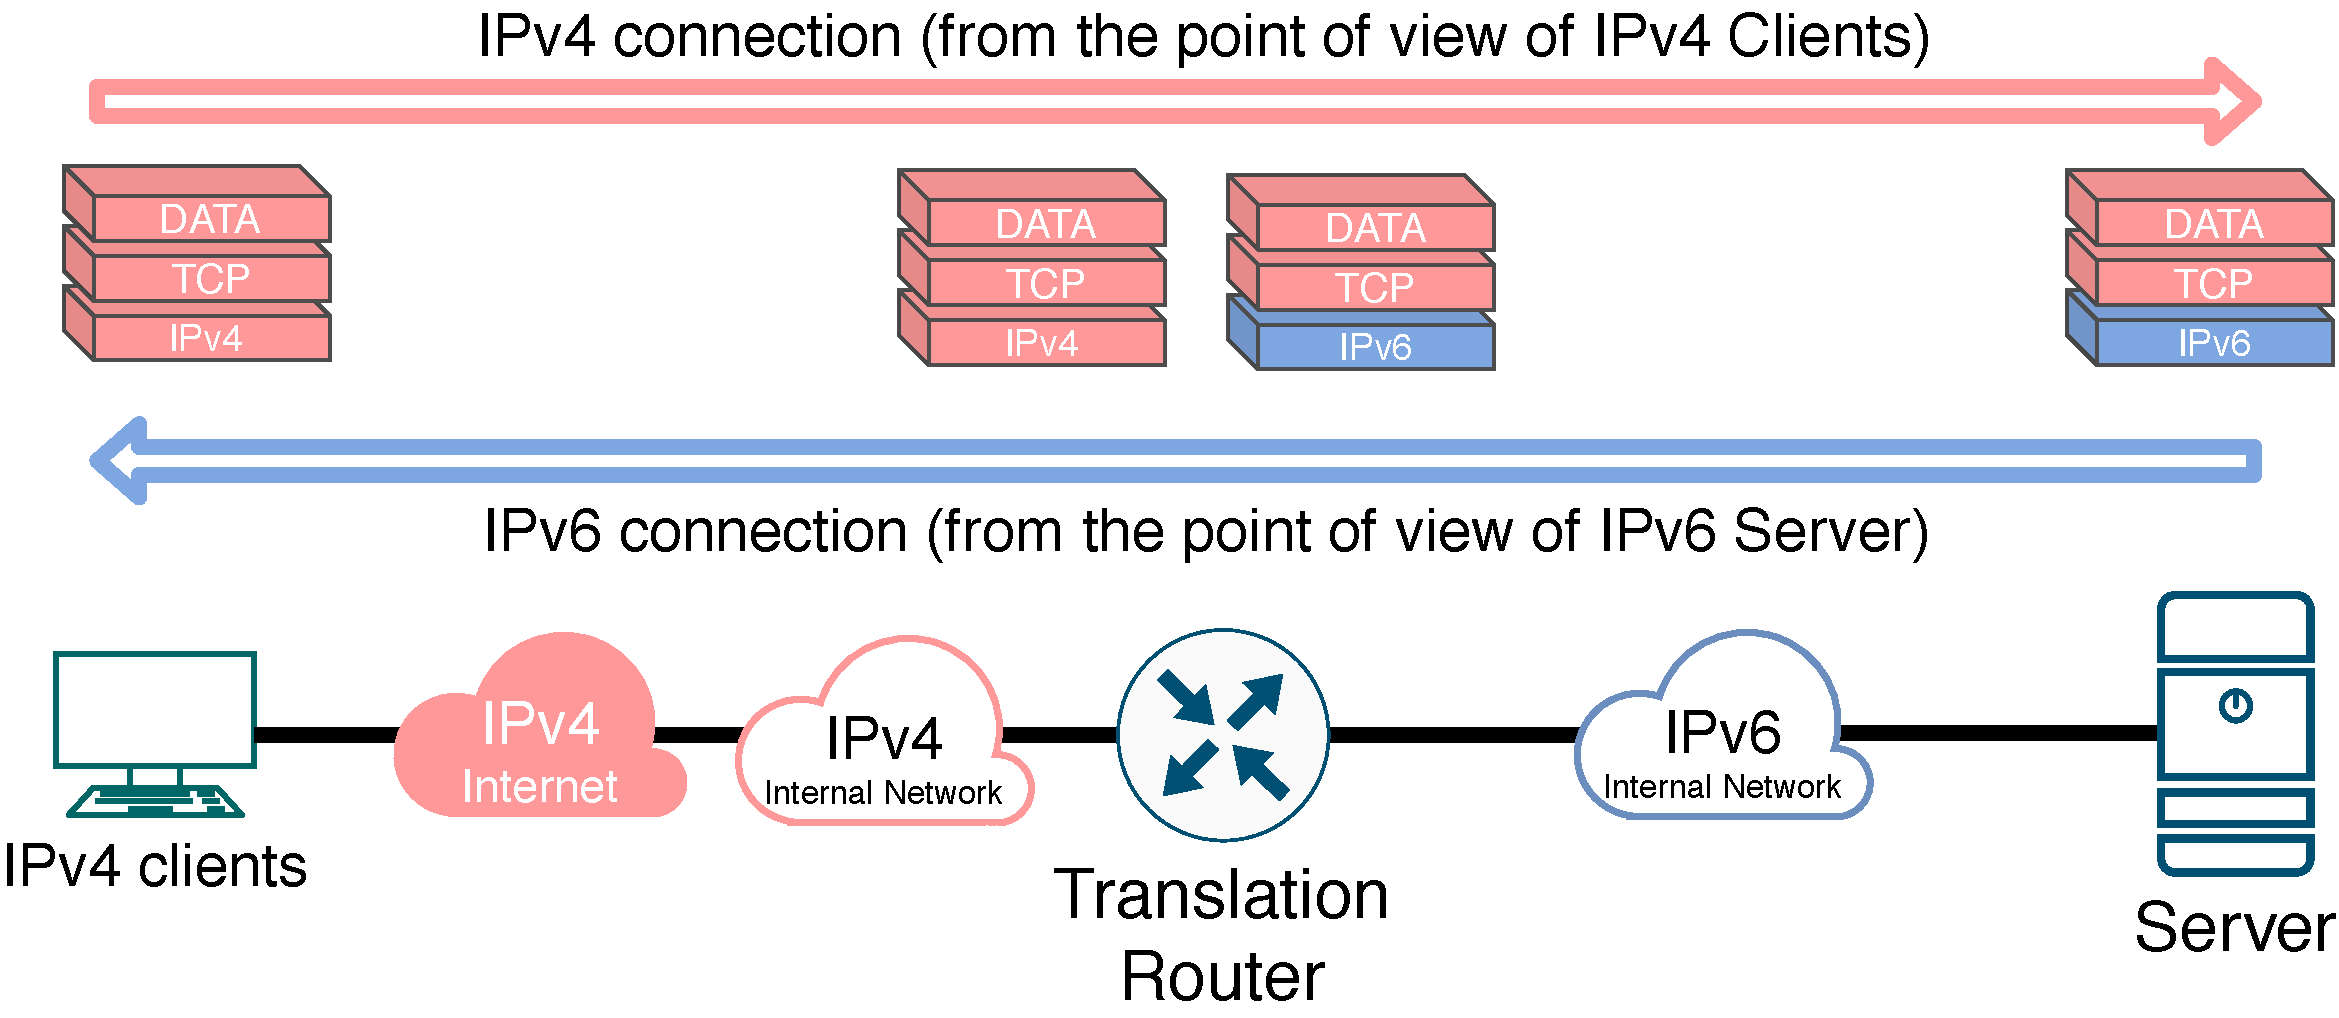
\includegraphics[width=15cm,pagebox=cropbox,clip]{img/translation_model.pdf}
    \end{center}
    \caption{IPv4/IPv6トランスレーションによるIPv4サービス提供}
    \label{fig:tunneling_model}
\end{figure}

IPv4/IPv6トランスレーションとは,IPv4パケットとIPv6パケットをIP/ICMP変換アルゴリズムを利用して相互に変換する手法である.$1:N$の関係でアドレス・ポート変換を行うステートフルなNAT64\cite{RFC6146}と,$1:1$でアドレス変換を行うステートレスなSIIT\cite{RFC7915}が定義されている.IPv4ネットワークとIPv6ネットワークの境界に位置する変換ルータにより,相互にプロトコル変換が行われる.

IPv4/IPv6トランスレーションではIPv4アドレスをIPv6アドレスとして表現することが要求されるが,変換プレフィックスと呼ばれるIPv6ネットワークプレフィックスにIPv4アドレスを埋め込むことで,任意のIPv4アドレスをIPv6ホストから認識可能な形で表現する.変換プレフィックスにはRFC6052で定義された64:ff9b::/96の他に,運用者が専有可能なGUA(Global Unicast Address)の/96のIPv6プレフィックスを利用することが想定されている\cite{RFC6052}.

図\ref{fig:tunneling_model}で示すように,変換ルータ以外のホストがIPv4ネットワークに属する必要が無いため,第\ref{related:abstract:requirements}項で述べた「IPv4ネットワークへの非依存性」の面で,他の2手法より優れていると言える.また,IPv4サービスを行うサーバから変換ルータの間はネイティブなIPv6ネットワークで接続可能なため,ECMP(Equal Cost Multi Path)\cite{rfc2992}による経路の冗長化が可能なほか,ステートレスモードでは変換ルータのスケールアウトが可能な点で,IPv6シングルスタックネットワークにおけるIPv4サービス提供に求められる要件を満たしやすい.

またサーバ側においても,アクセスコントロールの設定やログデータの管理など,IPv4とIPv6で別個に行われていた制御の削減が期待される.サーバ・アプリケーション管理者はネットワークプロトコルを意識したオペレーションをする必要がなく,運用効率改善の点でメリットが非常に大きい.

一方でIPv4とIPv6のプロトコル実装に差があるため,コンテンツ事業者のサービスの内容によってはサービス影響を考慮する必要がある点は留意すべきである.


\section{本章のまとめ}
\ref{related:abstract:requirements}項で述べた評価要件を尺度として,各IPv4サービス提供手法の特徴を比較した図を\ref{table:related_compare}に示す.

基本的なIPv4サービス提供手法の必要要件であるIPv4クライアントからのアクセスは各手法とも充足可能な一方,スケーラビリティの面では1:1/1:Mの接続が必須になるIPv4/IPv6トンネリング手法が他の手法から大きく劣る.
またL7リバースプロキシ手法はスケールアウト可能なアーキテクチャであるが,L4LB及びプロキシサーバLまでIPv4ネットワークを配備する必要があるため,IPv4ネットワークへの依存性が大きい.

IPv4/IPv6トランスレーション手法はスケールアウトが可能であり,IPv4ネットワークへの依存性が小さいため,IPv6シングルスタックネットワーク環境でのIPv4サービス提供手法として最も要件に適合する.


\begin{table}[h]
  \label{table:related_compare}
  \caption{IPv4サービス提供手法の比較}
  \centering
  \resizebox{\textwidth}{!}{%
  \begin{tabular}{lccc}
  \hline
  \multicolumn{1}{c}{手法名} & IPv4クライアントからのアクセス & \multicolumn{1}{l}{スケーラビリティ} & \multicolumn{1}{l}{IPv4ネットワークへの依存性} \\ \hline
  (参考)IPv4/IPv6デュアルスタック & 可能 & 困難 & 大 \\
  L7 リバースプロキシ & 可能 & スケールアウト可 & 中 \\
  IPv4/IPv6 トンネリング & 可能 & 困難 & 中 \\
  IPv4/IPv6 トランスレーション & 可能 & スケールアウト可 & 小 \\ \hline
  \end{tabular}%
  }
\end{table}
%%% Local Variables:
%%% mode: japanese-latex
%%% TeX-master: "../thesis"
%%% End:
\chapter{データプレーン高速化に伴う課題}
\label{issue}
第\ref{related:compare:translation}項で述べたPv4/IPv6トランスレーションを用いたIPv4サービス提供手法の一つとして,SIIT-DCがインターネット標準化されている.
本章ではSIIT-DCのデザインとメリット及び考えられる運用,そして現状の課題について述べる.
\section{SIIT-DC}
\label{issue:siit-dc}


% \subsection{概要}
% SIIT-DCとは,ステートレスIP/ICMP変換アルゴリズム\cite{RFC7915}を利用して,IPv4インターネット・ネットワークからのアクセスをIPv6シングルスタックネットワーク上のホストに提供するためのネットワークデザインである.2016年にIETF IPv6 Operations WG\footnote{IPv6ネットワークの運用要件や関連する技術仕様の策定を行うワーキンググループ.\url{https://datatracker.ietf.org/wg/v6ops/about/}}での議論を基にRFC7757として標準化された\cite{RFC7755}.


% \subsection{用語}
% \label{issue:siit-dc:terms}
% SIIT-DCで利用される用語,及び特徴的な役割を有する機器・技術について述べる.

% \subsubsection{SIIT(Stateless IP/ICMP Translation Algorithm)}
% SIITとはIPv4/IPv6トランスレーションに用いられるプロトコル変換機能の略称である.RFC2765\cite{RFC2765}で初めて標準化され,その後RFC6145\cite{RFC6145}により一部の仕様が実運用のユースケースに合わせて変更された.現在はIPv6拡張ヘッダーを扱う機構などが追加されたRFC7915\cite{RFC7915}が現行の標準仕様である.

% \subsubsection{BR(Border Relay)}
% BRとは,SIIT-DCネットワークにおいてIPv4インターネットとIPv6ネットワークとの間でSIITによるIPv4/IPv6トランスレーションを行う機器もしくは他の役割を有する機器の一機構である.
% IPv4インターネットとIDC内のIPv6シングルスタックネットワークの各境界部に所在し,後述するEAMTを参照した1:1のアドレス変換を行う.IDCネットワークにIPv4インターネットとの接続点が複数ある場合,接続点ごとに最低一つのBRを配備する.

% \subsubsection{ER(Edge Relay)}
% ERとは,IDC内のIPv4ネットワークとIPv6ネットワーク間での多:多のIPv4/IPv6トランスレーションを行う機器である.

% SIIT-DCではそのオプションとして,IPv4ネットワーク内のIPv4しか利用出来ないホストが,SIIT-DCを利用してIPv4サービスを提供するユースケースをサポートするSIIT-DC Dual Translation Mode\cite{RFC7756}が定義されており,ERはその中での利用が想定されている.

% 通常,ERが有する後述のEAMTはIDCネットワーク内のIPv4ネットワークアドレスと,そのIPv4ネットワークを示すIPv6サービスアドレスにより構成される.

% \subsubsection{IPv4サービスアドレス}
% IPv4サービスを提供するIPv6シングルスタックネットワークに属するホストに割り当てるIPv4アドレス(群)をIPv4サービスアドレスと呼称する.
% このアドレス宛に送信されたパケットは,BR/ERによって対応するIPv6サービスアドレスに変換される.

% なお,IPv4サービスアドレスはIPv4インターネットに経路広告されている必要がある.

% \subsubsection{IPv6サービスアドレス}
% ER/BRを介してアプリケーションやホストに割り当てられたIPv6アドレス(群)をIPv6サービスアドレスと呼称する.
% IPv4クライアントはSIIT-DCのアーキテクチャをを通じて,このIPv6サービスアドレスが割り当てられたホストと通信することが出来る.

% \subsubsection{変換プレフィックス}
% \label{issue:siit-dc:translation-prefix}
 
% 変換プレフィックス(Translation Prefix)とは,全てのIPv4アドレスをマッピングするために用いられる,プレフィックス長が96bitのIPv6ネットワークプレフィックスである\cite{RFC6052}.IANAによって主にWKP(Well Known Prefix)として64:ff9b::/48が予約\cite{RFC8215,IANA_allocation_v6}されているが,運用者の裁量でISP自身に割り当てられたNSP(Network Specific Prefx)\footnote{主にRIRから割り当てられたIPv6 Global Unicas Addressを指す.}を利用する事ができる.

% IPv4アドレスとIPv6アドレスの間で変換を実行する際に,BR/ERは変換前のIPヘッダーのアドレスフィールドを、変換プレフィックスが挿入・削除された状態に書き換える。

% なおSIIT-DCネットワークにおいて,変換プレフィックス宛のパケットは各BR/ERのIPv6インターフェース宛にIGP(Interior Gateway Protocol)などで経路広告される必要がある.

% \subsubsection{EAM(Ecplicit Address Mapping)/EAMT(Ecplicit Address Mapping Table)}
% EAMとは,EAMアルゴリズム\cite{RFC7757}によって結びつけられたIPv4サービスアドレスとIPv6サービスアドレスのペアを表す.

% EAMにおいて,それぞれ同数のIPv4サービスアドレスとIPv6サービスアドレスによって構成される.標準では結び付けられたIPv6サービスアドレスがIPv4サービスアドレスより多い状態が想定されているが,IPv6サービスアドレスのホスト部が若いものから優先して変換するため,余剰分のアドレスは無視される.

% また,BR及びERが変換を行う際に参照するEAM群が記録されたテーブルをEAMTと定義している.以後EAMTもしくは変換テーブルと呼称する.



% \subsection{ネットワーク設計}
% \label{issue:siit-dc:network}
% \begin{figure}[h]
%     \begin{center}
%       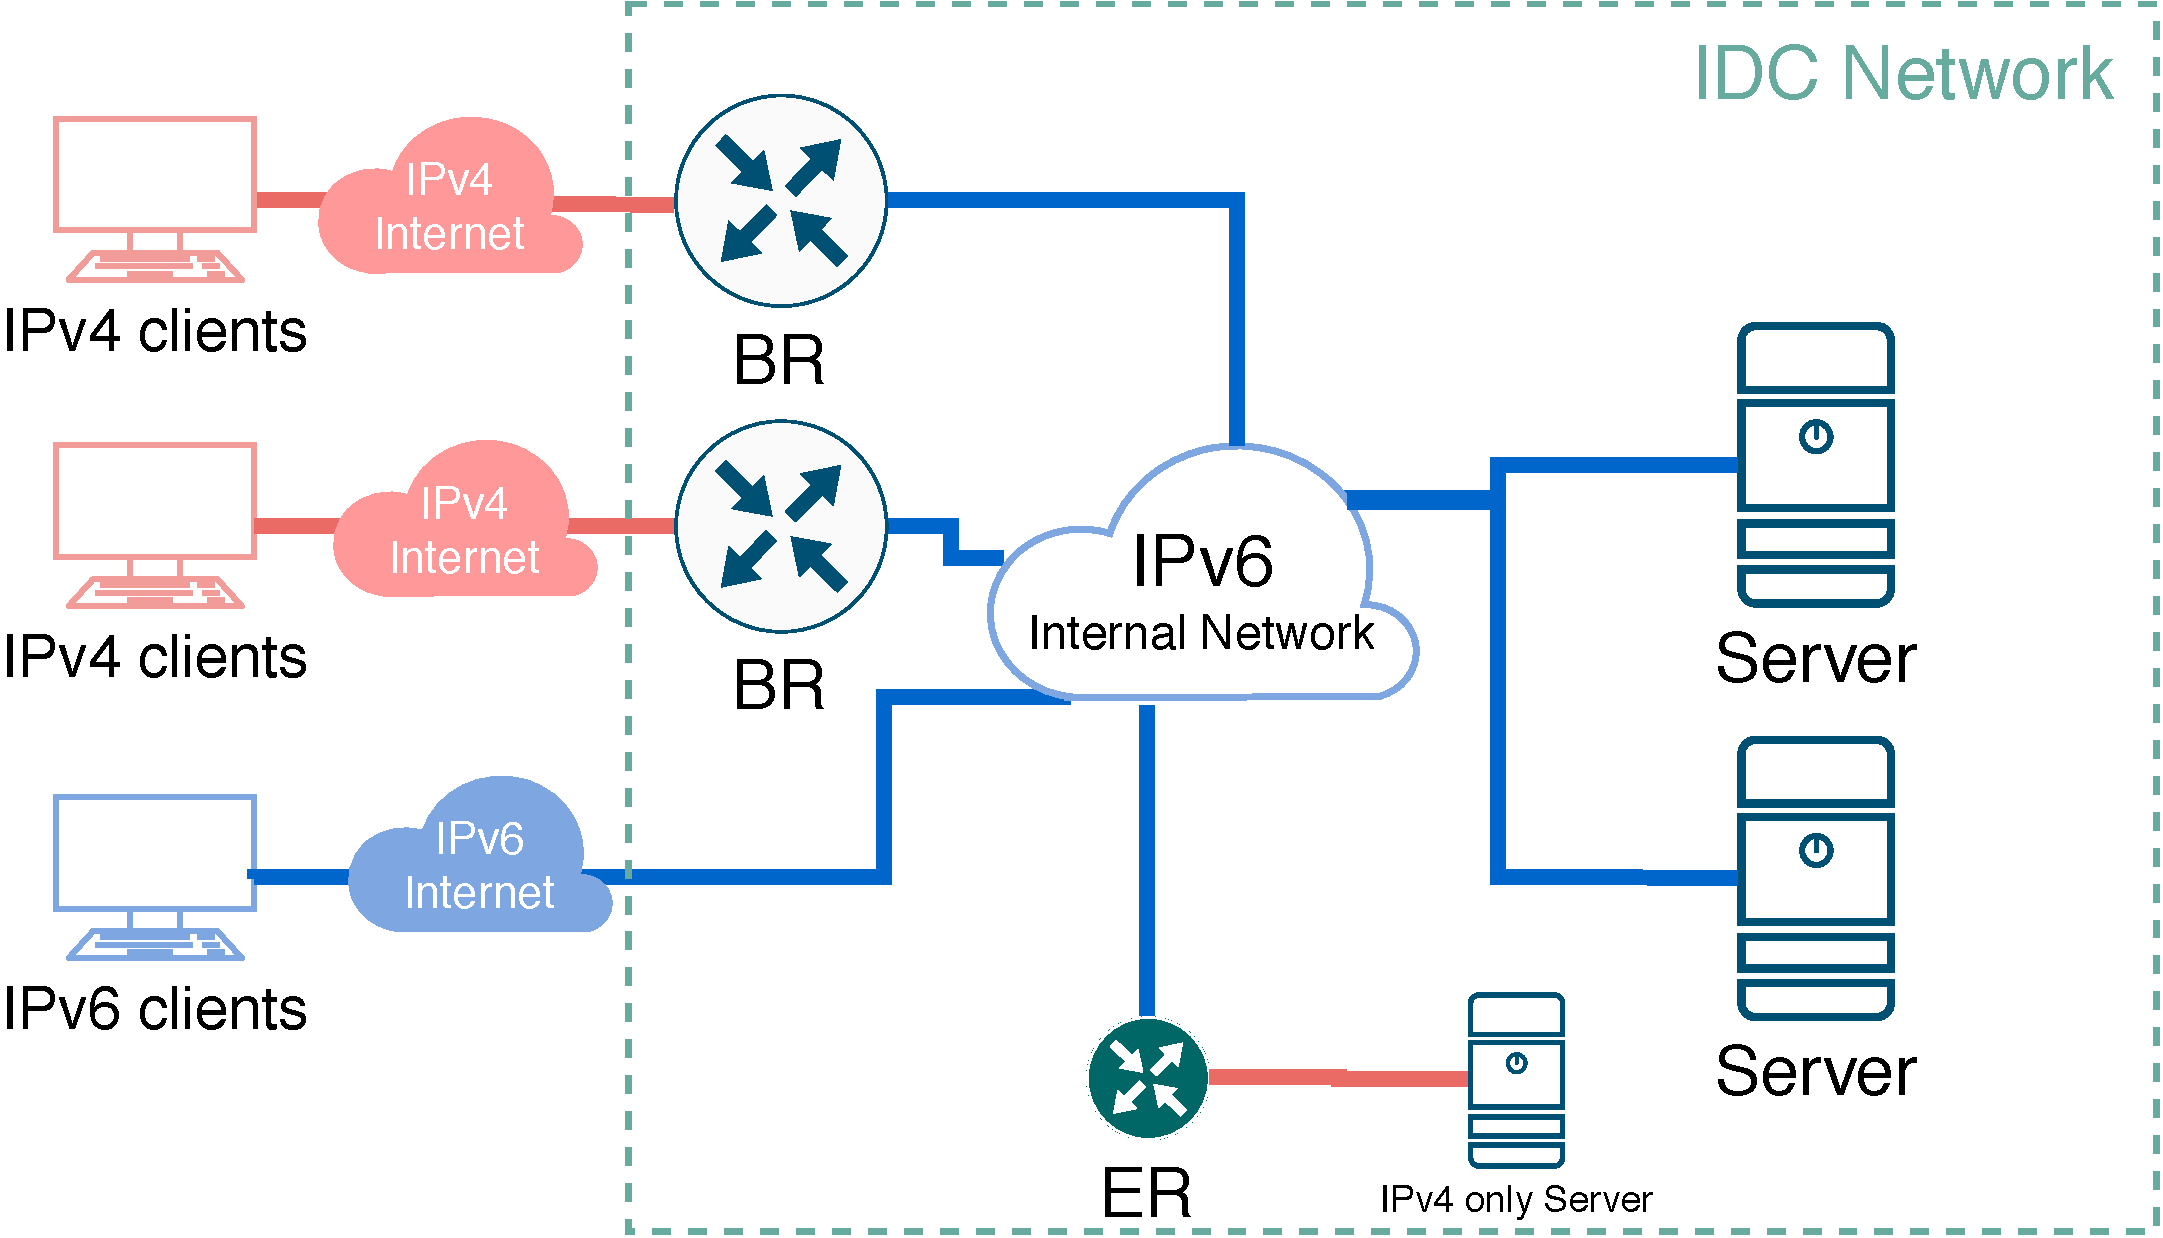
\includegraphics[width=12cm,pagebox=cropbox,clip]{img/siit-dc-network.pdf}
%     \end{center}
%     \caption{SIIT-DC ネットワーク}
%     \label{fig:siit-dc_network}
% \end{figure}
% 基本的なSIIT-DCネットワークを図\ref{fig:siit-dc_network}に示す.

% BRはIPv4インターネットとの各接続点に配置される.各IPv4サービスアドレスは自組織のアドレスとして,IPv4インターネットに経路広告される必要がある.

% SIIT-DCネットワークでは,変換プレフィックス宛のパケットはBRに対してルーティングされる.
% BRが複数ある場合,BRがネットワークプロトコルに利用する変換プレフィックスを別個に用意するか,同一の変換プレフィックスを各BRにエニーキャスト\cite{RFC4786}によってルーティングさせる.エニーキャストを使用した場合,BRの障害時には別のBRへとトラフィックを迂回させることが可能である.

% ERはIDC内のIPv4ネットワークとの接続点に配置され,IPv4のみを持つホストがIDC内のIPv6ネットワークを介してIPv4インターネットにサービス提供を行う場合に利用される.


% \subsection{SII-DCのメリット}
% \label{issue:siit-dc-merit}
% SIIT-DCを用いたIPv4サービスの提供によるメリットとして,以下の点が挙げられる,

% \subsubsection{デプロイメントが容易}
% SIIT-DCでは,IDCのIPv6ネットワークとIPv4インターネットとの接続点にBRを設置を行うのみにより,基本的なIPv4サービスの提供が可能である.
% そのためIDCのネットワークトポロジに限定されないシンプルなIPv4サービス提供が期待できる.

% \subsubsection{アドレス単位でのIPv4アドレスの効率的な利用が可能}
% 通常のIPネットワークにおいて,サーバに対するIPアドレスアサインメントはサブネット単位での割り当てを行う必要がある.従来,事前に同一サブネットに属するホスト数を見積持った上で不足が生じないようにネットワークサイズを設定する必要があるめ,ネットワークサイズを超えるサービスの拡大が必要になった場合,サブネット全体の再設計が不可欠であった.またIPネットワークには,ネットワークアドレスやブロードキャストアドレス,そしてデフォルトゲートウェイとなるルータのインターフェースのアドレスを確保する必要があり,ネットワークサイズが断片化されるほど,実質的に利用できないアドレスの割合が大きくなる問題が会った.

% しかしながらSIIT-DCではサーバごとにアドレスを割り当てることが出来るため,従来利用できなかったIPv4アドレスを再利用することで,IPv4アドレスの効率的な利用を実現できる.第\ref{introduction:background:ipv4_problems}項で述べたように今後益々IPv4アドレスの調達が困難になることが予想されるため,IPv4アドレスの効率的な利用は事業者の負担軽減に繋がる.

% \subsubsection{スケーラビリティ}
% \label{issue:siit-dc-merit:scalability}
% \begin{figure}[h]
%   \begin{center}
%     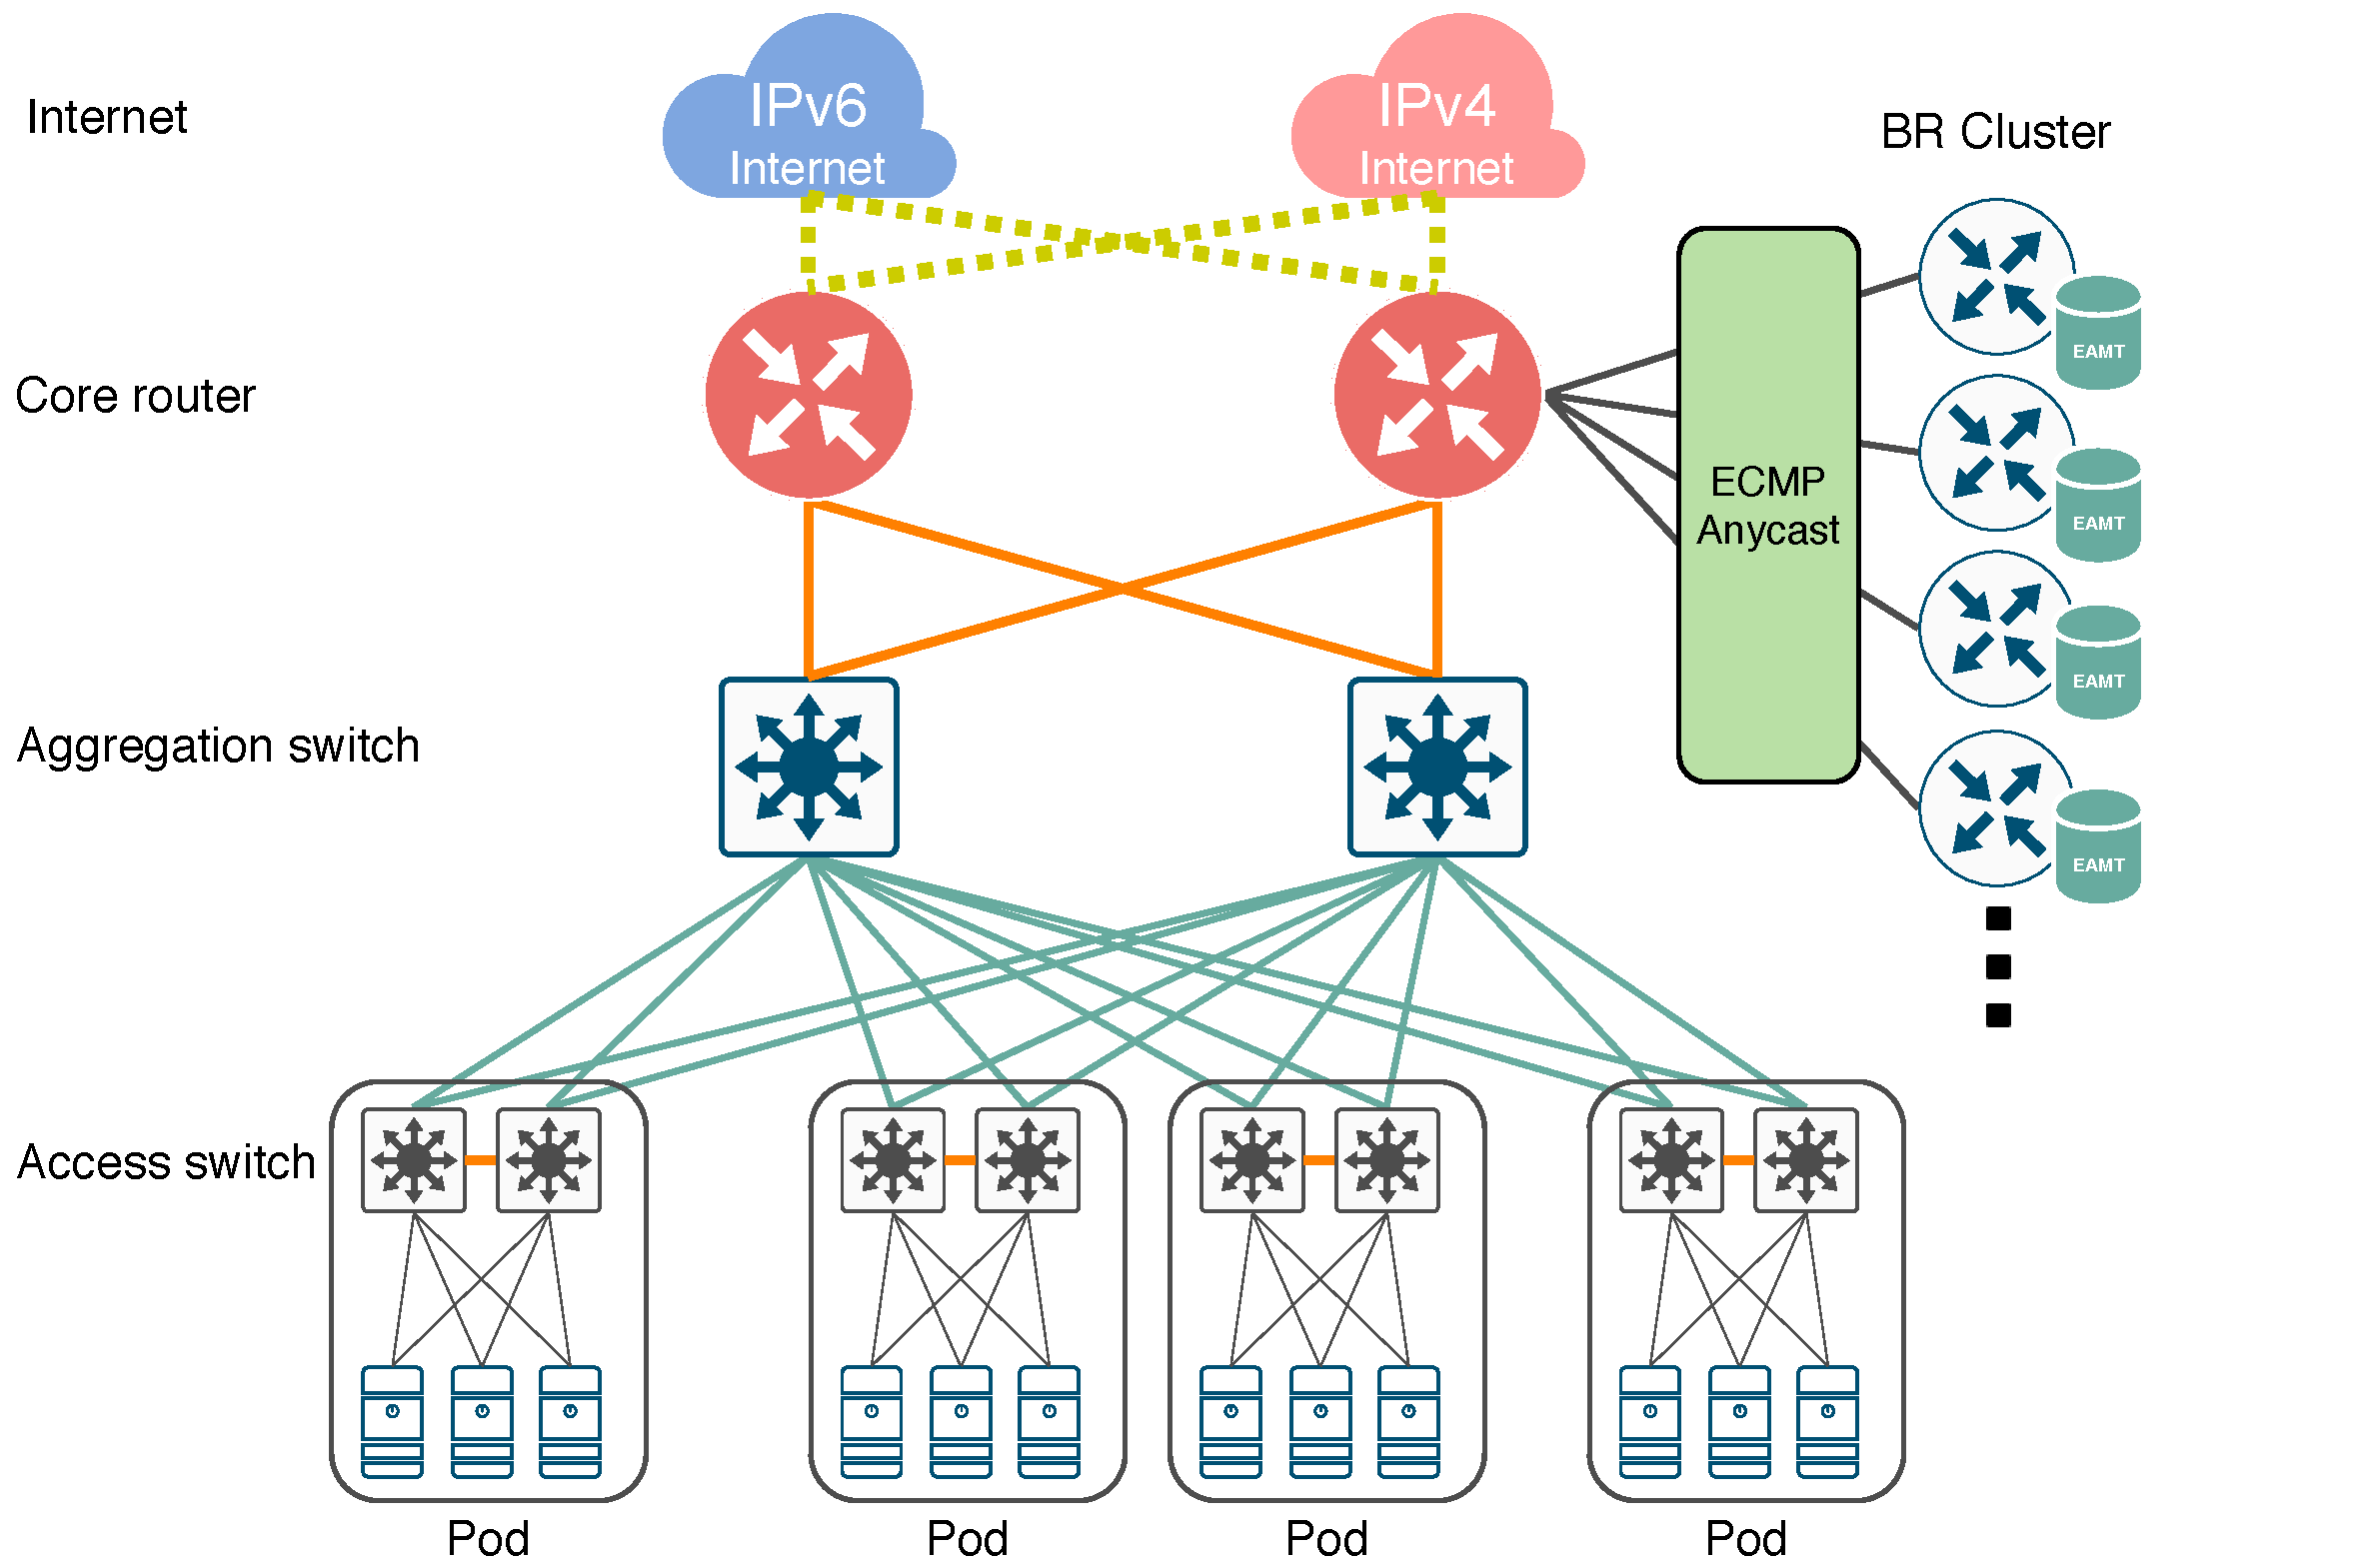
\includegraphics[width=12cm,pagebox=cropbox,clip]{img/siit-dc_scale.pdf}
%   \end{center}
%   \caption{BRを水平スケールすることが出来るSIIT-DCネットワーク}
%   \label{fig:siit-dc_network_scale}
% \end{figure}
% SIIT-DCの標準仕様\cite{RFC7755}では明示的に述べられていないが,本論文ではBRを並行して複数配置することで,スケールアウトが可能なネットワークデザインを立案する.
% 本ネットワークデザインでは,ECMP及びエニーキャスト\cite{RFC4786}を利用することにより,BRの数を水平に増加させることで,IPv4サービスの提供容量をリニアに増加させることが可能である.

% 図\ref{fig:siit-dc_network_scale}に本ネットワークデザインに則ってBR配置を行ったスケーラブルなSIIT-DCネットワークの例を示す.IPv4クライアントからのアクセスはいずれかのBRにフォワーディングされた後,IPv6プロトコルに変換された上で再度コアルータを介してIDCネットワーク内のIPv4サービス提供サーバに到達する.



% \subsection{基本的なパケットの流れ}
% \label{issue:siit-dc:packet_flow}

% \begin{figure}[h]
%     \begin{center}
%       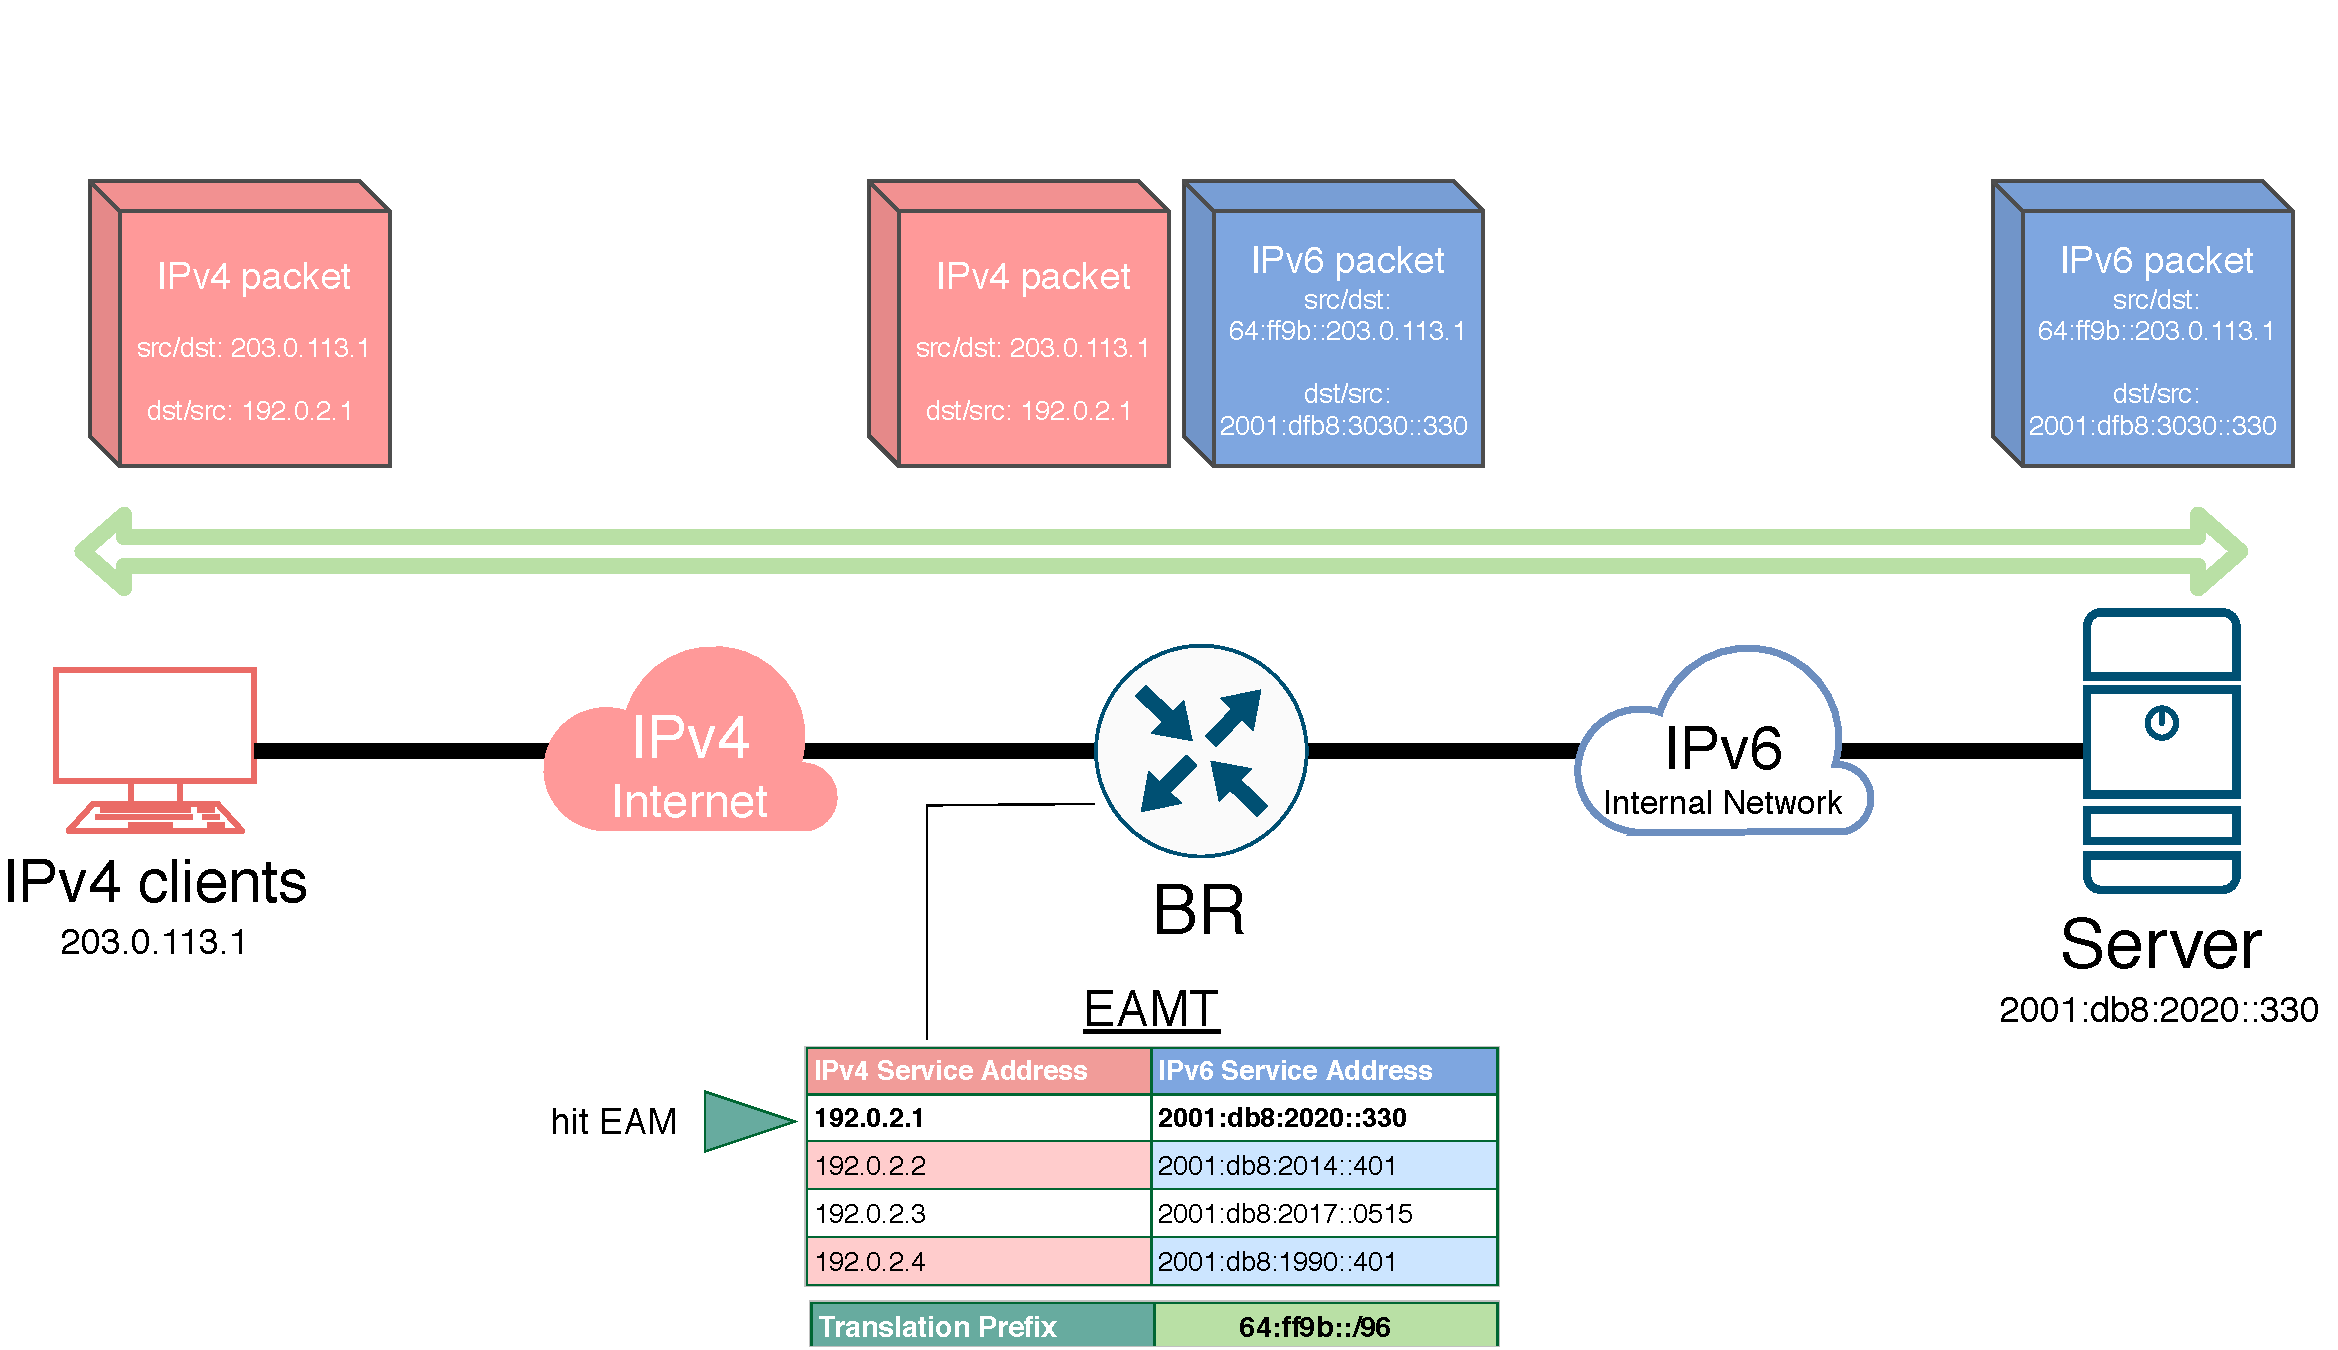
\includegraphics[width=14cm,pagebox=cropbox,clip]{img/siit-dc_packet.pdf}
%     \end{center}
%     \caption{SIIT-DC パケットの流れ}
%     \label{fig:siit-dc_packet}
% \end{figure}

% SIIT-DCにおける基本的なIPv4クライアントからのトラフィックの流れは以下の様になる.一連のパケットの送信元・送信先のアドレスの遷移を図\ref{fig:siit-dc_packet}に示す.

% IPv4クライアントのIPv4サービスアドレス宛のパケットはIPv4インターネットに接続するBRに到達後,当該BRが有するEAMTに従ってIPv6サービスアドレス宛のIPv6パケットに変換される.このパケットの送信元アドレスは変換プレフィックスに埋め込まれたIPv6アドレスとして表現される.IDC内のIPv6ネットワークを介してIPv6サーバに到達した後,IPv6サーバは送信元アドレスへの応答パケットを送信する.\ref{issue:siit-dc:translation-prefix}項で述べたように,変換プレフィックス宛のパケットはIPv6ネットワークを経由してBRにルーティングされる.IPv6サーバからの応答を受け取ったBRはEAMTを参照し,送信元アドレス(IPv6サービスアドレス)をIPv4サービスアドレスに書き換え,送信先アドレス(IPv4クライアントのIPv4アドレス)から変換プレフィックスを除去書き換えたのち,IPv4インターネットを介してIPv4クライアントに返送される.




% \section{SIIT-DCの課題}
% \label{issue:siit-dc_problems}
% 本節ではSIIT-DCの現状の課題及びそれに起因して起こる事象に関して述べる.

% \subsection{一貫したEAMTの必要性}
% \label{issue:siit-dc_problems:consistent}

% \begin{figure}[h]
%     \begin{center}
%       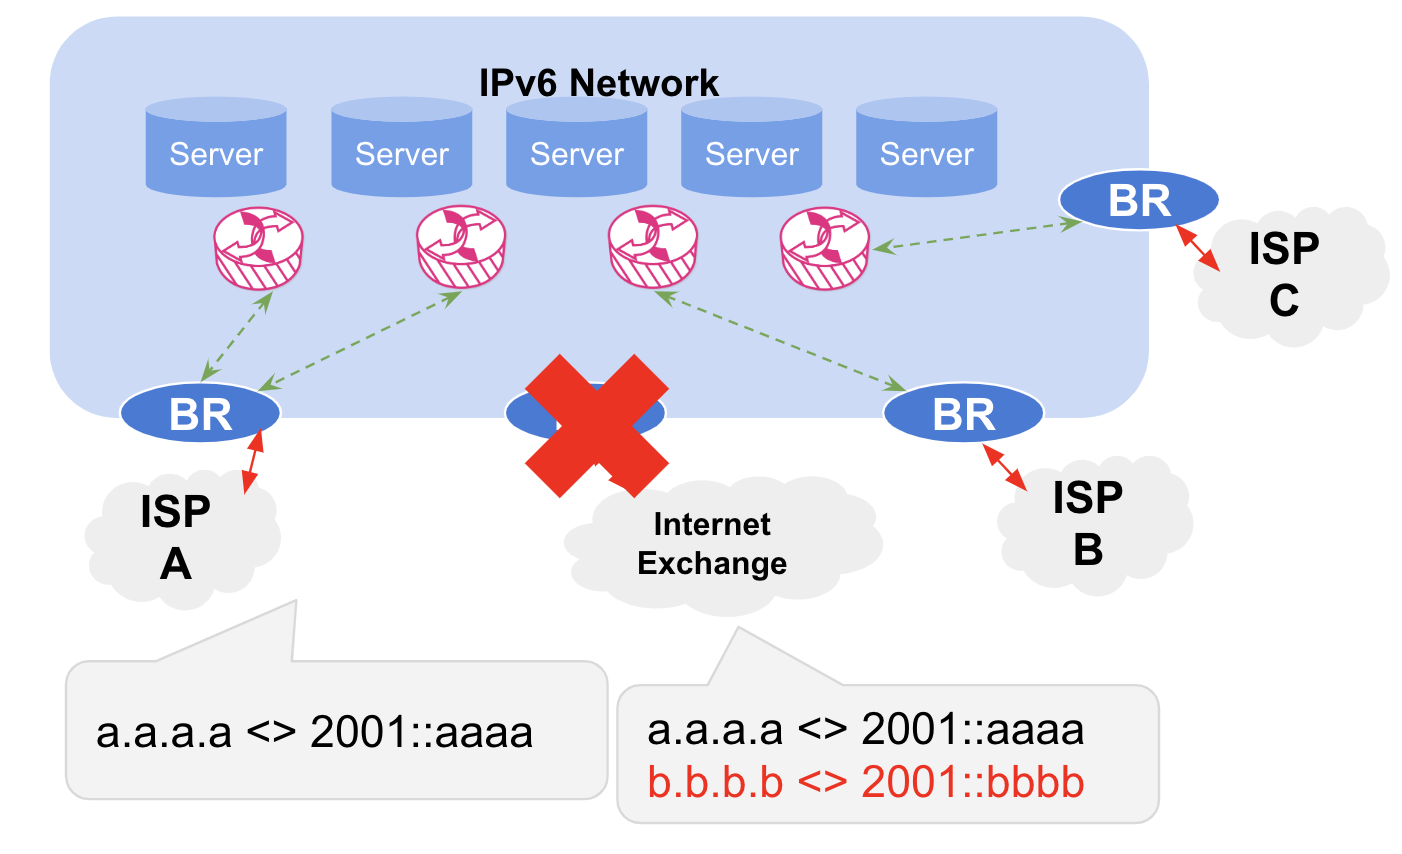
\includegraphics[width=10cm,pagebox=cropbox,clip]{img/siit-dc_can-not-failover.png}
%     \end{center}
%     \caption{BRに障害が発生した場合に適切にフェイルオーバーが出来ないケース}
%     \label{fig:siit-dc_can-not-failover}
% \end{figure}

% \ref{issue:siit-dc:terms}項で述べたように,SIIT-DCでは対外接続点ごとにBRを配置するネットワークデザインを採用することで,IPv6シングルスタックネットワークに最小限のIPv4ネットワークを追加するだけでIPv4サービスの提供を可能にしている.また\ref{issue:siit-dc:network}項や\ref{issue:siit-dc-merit:scalability}項で触れたように,複数のBRで共通した変換プレフィックスをエニーキャストでIDCネットワーク内に広告する運用を行うことにより,BR及び対外接続点の障害時に他のBRを用いてIPv4サービスの提供を継続することが出来る.この機構を有効に作用させるためには,SIIT-DCネットワーク内の全てのBRで一貫したEAMTの保持が求められる.

% しかしながら現状のSIIT-DC及びEAMTの仕様\cite{RFC7755,RFC7756,RFC7757}では,BRは他のBRとの間でEAMTを共有するためのメッセージング機構を有さない,これはBR間でEAMTの不一致が発生した場合に,差異となったEAMに該当するIPv4サービス宛のトラフィックを別のBRへ迂回出来なくなるケースが発生することを意味する.


% \subsection{変更追従性の欠如}
% \label{issue:siit-dc_problems:follow}

% \begin{figure}[h]
%     \begin{center}
%       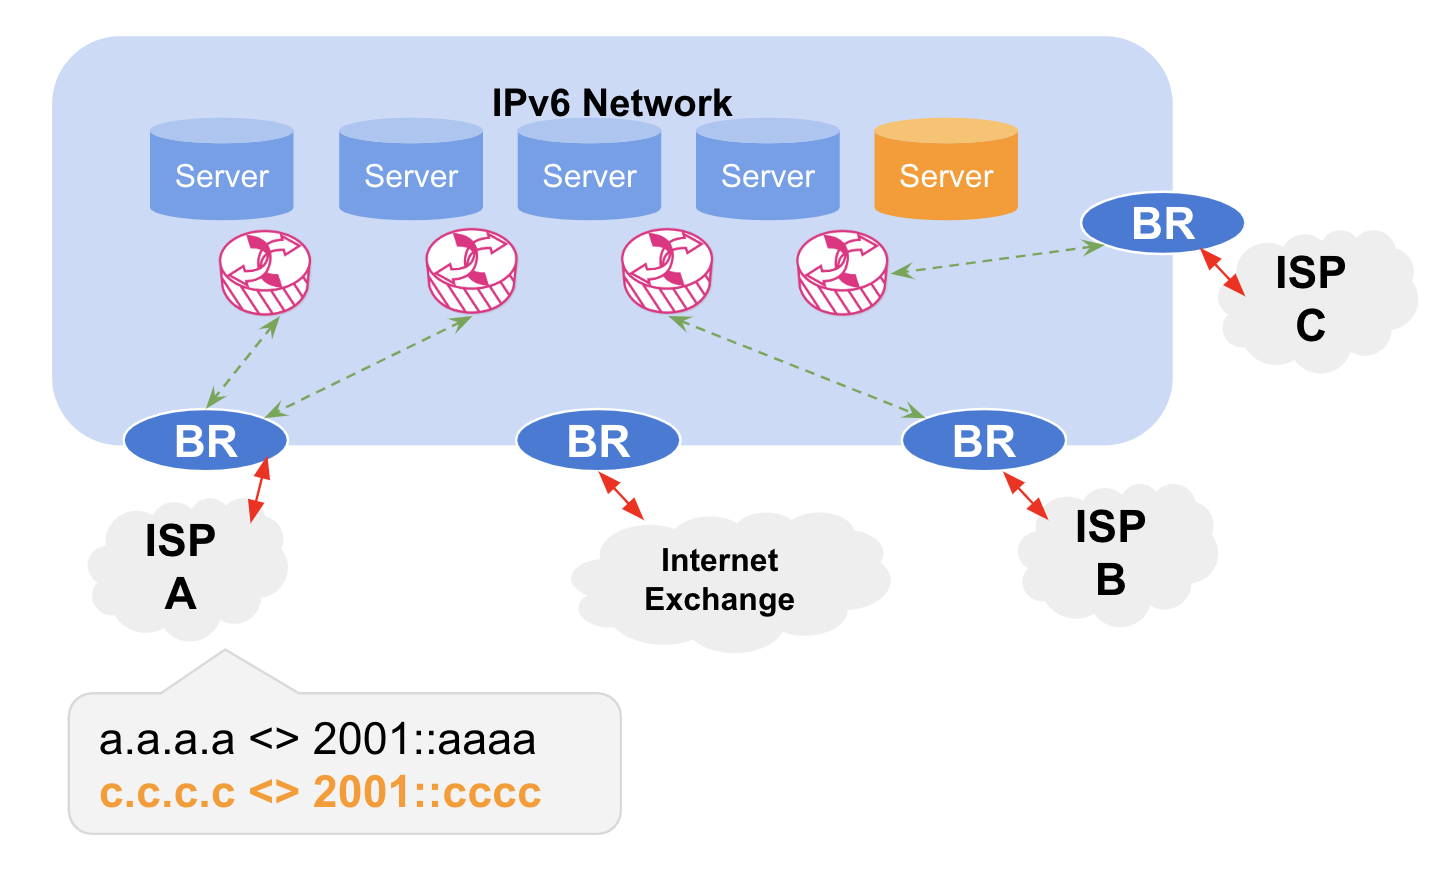
\includegraphics[width=10cm,pagebox=cropbox,clip]{img/siit-dc_add-server.png}
%     \end{center}
%     \caption{サーバを追加した際,全てのBRへの設定追加が必要になる.}
%     \label{fig:siit-dc_add-server}
% \end{figure}

% プライベートクラウド環境が一般的に利用されるIDCネットワークでは,日々多くのサーバやアプリケーションが追加・廃止・変更される.
% 一方で\ref{issue:siit-dc_problems:consistent}項で触れたように,SIIT-DCでIPv4提供サービスを冗長に運用するためには,IPv4提供サービスに該当するEAMがBRのEAMTに保持されることが要求される.IPv4提供サービスの構成に変更があった場合,全てのBRのEAMTを更新する必要がある.

% しかしながら現状SIIT-DC及びEAMTの仕様\cite{RFC7755,RFC7756,RFC7757}において,IPv4サービスを行うサーバの存在や状態によってダイナミックにEAMTを更新する機構は存在しない.そのため,IDCネットワークにおけるIGPなどによってIPv6サービスへの到達性が検証されていたとしても,IPv4サービスの場合はリアルタイムな構成変更に追従することが出来ない.


% \section{本章のまとめ}
% 第\ref{issue:siit-dc_problems}項で述べたように,現状のSIIT-DC及びEAMTの仕様はEAMTの一貫性を担保する手法の検討がなされておらず,それに起因した障害時の適切なフェイルオーバーの実行やIPv4サービスの増減時の変更追従に関しての課題がある.
% NPO日本ネットワークセキュリティ協会(JNSA)らの調査によればITシステムの障害の原因の約半数は人為ミスに分類されるものにあり\cite{human_error},サービスの安定的な稼働を実現するためには単調な繰り返し動作を含む運用をシステムによって減らす必要がある.


%%% Local Variables:
%%% mode: japanese-latex
%%% TeX-master: "./thesis"
%%% End:

\chapter{手法の検討}
\label{consideration}

\section{概要}
第\ref{issue:siit-dc_problems}項で述べたように,現状のSIIT-DC及びEAMTの仕様はEAMTの一貫性を担保する手法の検討がなされておらず,それに起因した障害時の適切なフェイルオーバーの実行やIPv4サービスの増減時の変更追従に関しての課題がある.
NPO日本ネットワークセキュリティ協会(JNSA)らの調査によればITシステムの障害の原因の約半数は人為ミスに分類されるものにあり\cite{human_error},サービスの安定的な稼働を実現するためには単調な繰り返し動作を含む運用をシステムによって減らす必要がある.

本研究ではSIIT-DCにおけるダイナミックEAMT\footnote{BR群のEAMTをシステムにより動的に制御する機構}の実現を目指す.本章では考えられる手法を大別した上でその特徴と利点及び欠点を挙げ,最も適した手法を検討する.


\section{求められる要件}
\label{consideration:points}

第\ref{related:abstract:requirements}で述べたIPv4サービス提供手法の機能要件と,第\ref{issue:siit-dc_problems}項で挙げたSIIT-DCの現状の課題を総合し,EAMTを動的に制御する手法に求められる要件を下記のように定義した.

\subsubsection{BR間のEAMTの一貫性}
第\ref{issue:siit-dc_problems}項で述べたように,障害時の適切なフェイルオーバーを実現するためには,各BRのEAMTの一貫性が保証される必要がある.

\subsubsection{変更追従性}
近年のIDCでは多数の物理サーバーを統合的に管理するプライベートクラウド環境やコンテナオーケストレーション環境\footnote{Container Orchestration.コンテナ型仮想化統合管理環境}が普及しており,アプリケーション・サービスの追加及び削除が頻繁に行われている.サービスの障害時に適切にそれを検知し,適切に冗長系に移行するははSLB\footnote{Servver Load Balancer}を中心として広く利用されている.SIIT-DCのIPv4サービス提供の場でも,サービスの状態の変動にリニアに対応しフェイルオーバーできるような働きが求められる.

\subsubsection{スケーラビリティ}
第\ref{related:abstract:requirements}で述べたようにIPv6シングルスタックネットワークにおけるIPv4サービスの提供では水平スケールが容易に行える仕組みを備える必要がある.
IPv4サービスを行うサーバーの増設や,対外接続点が増えた場合のBRの拡大に十分に適用するスケーラビリティを有することが望ましい.

次項ではスケーラビリティの評価のために,制御に必要な通信コネクション数による比較を行う.以後BRの数を$M$,IPv4サービスを提供するサーバーの数を$N$とし,総通信コネクション数を$C$として表現する.


%
%\subsection{冗長性}
%EAMTを制御するために用いられる管理台帳となるデータは高可用性を有した形で保持する必要がある.EAMTを分散管理
%EAMTを制御するために用いられる管理台帳となるデータを保持するノードがいる場合,単一障害点になることを防ぐために高可用性クラスター\cite{gadir2005high}を構成できるアーキテクチャである必要がある.

\subsection{デプロイメントの容易さ}
第\ref{issue:siit-dc:network}で述べたように,SIIT-DCの最も特筆すべきメリットの一つにデプロイメントの容易さが挙げられる.
これを損なうこと無くダイナミックEAMTが導入されることが望ましい.


\section{アプローチの分類と比較}
\label{consideration:approach}
本説ではダイナミックEAMTを実現するアプローチとして,二系統のアプローチを考案する.それぞれのアプローチで考えられる実装と実際の構成,及び第\ref{consideration:points}節で述べた各要件への適合を定性的に評価する.



\subsection{中央管理型アプローチ}
\label{consideration:approach:centerized}

\begin{figure}[h]
    \begin{center}
      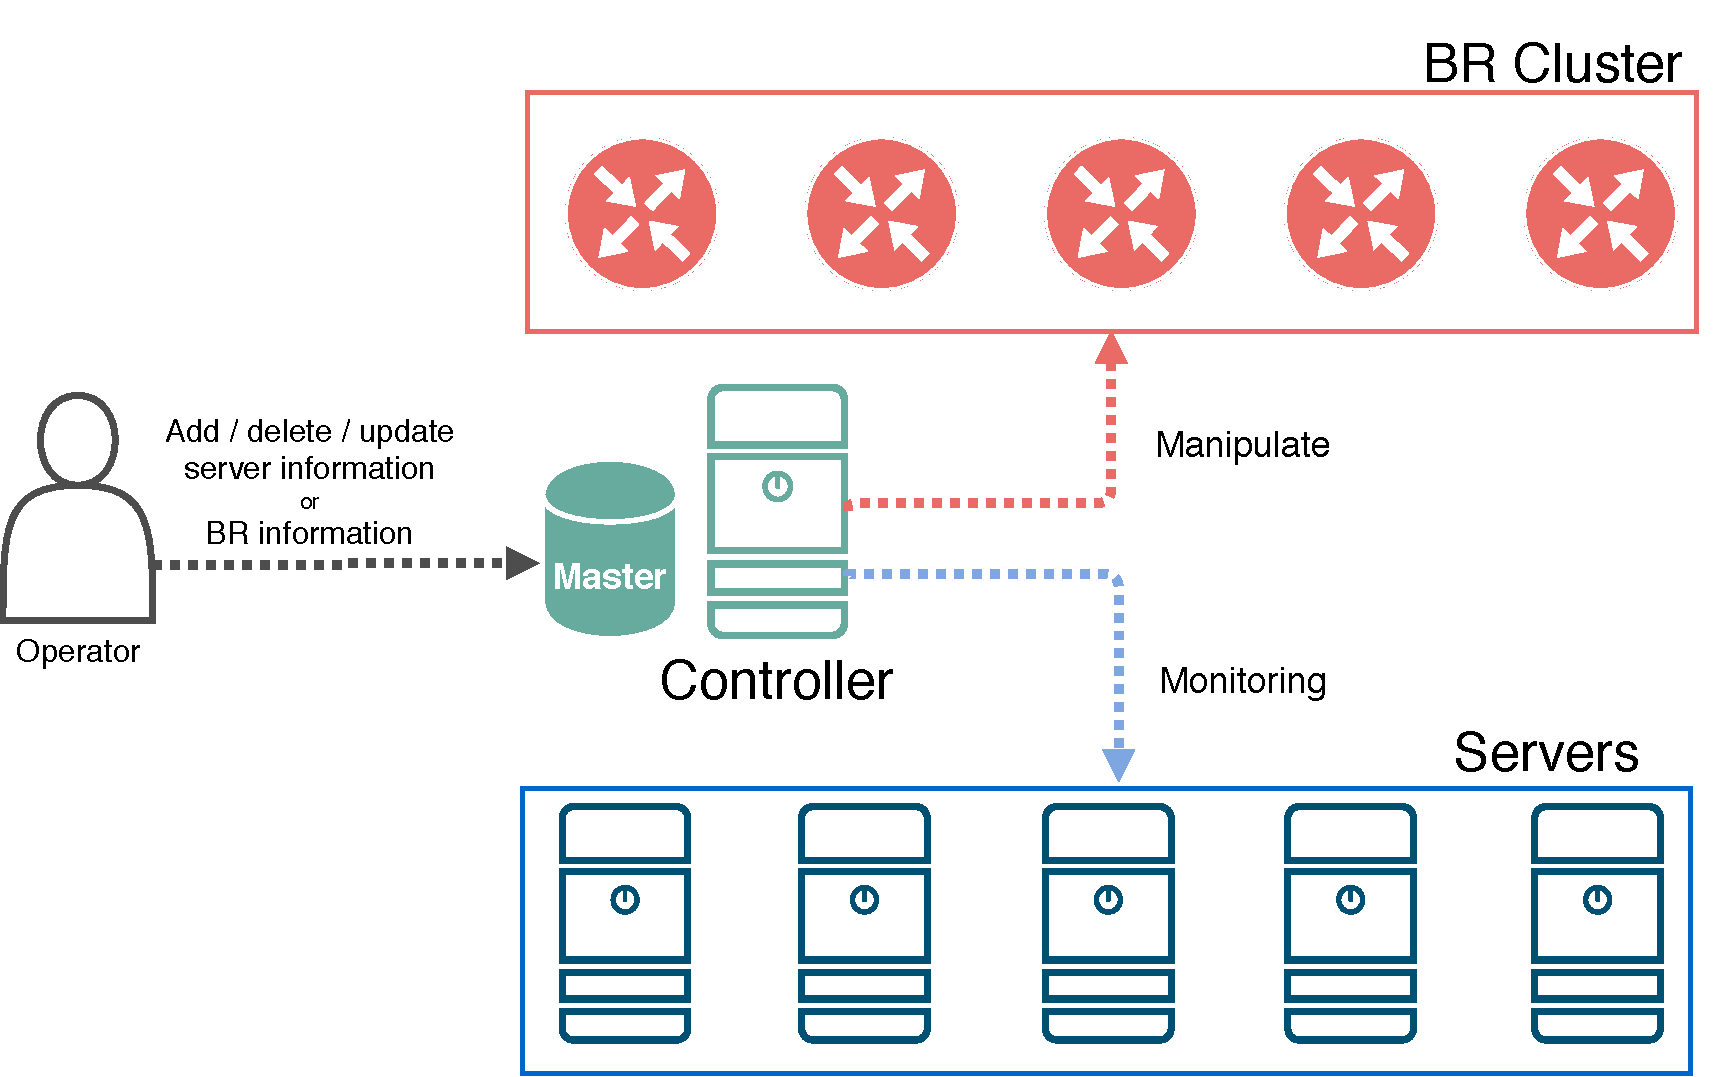
\includegraphics[width=12cm,pagebox=cropbox,clip]{img/approach_centerized_model.pdf}
    \end{center}
    \caption{中央管理型アプローチによるダイナミックEAMT}
    \label{fig:approach_centerized_model}
\end{figure}

中央管理型アプローチとは,複数のBRのEAMTを統合的に管理する「コントローラー」をIDCネットワーク上に配置し,各BRがネットワークを介してこれを参照する機構である.
図\ref{fig:approach_centerized_model}に中央管理型アプローチによってダイナミックEAMTを実現したSIIT-DCの各コンポーネントの関係図を表す.

中央管理型アプローチではコントローラーが各BRに投入するEAMが記録された「マスターテーブル」を保持し,それを元に各BRのデータプレーンにルールを書き込む手法を取る.マスターテーブルに記載されるEAMはオペレーターがネットワークの構成変更に合わせて追加・削除・更新を行い,それぞれのIPv4サービスを提供するサーバー群に対してはコントローラからプル型\footnote{pull-based monitoring. コントローラから各サーバーに能動的に情報を取得する}の外部監視\footnote{External monitoring}によりサーバーの状態変化を検知しマスターテーブルを更新する.

本アプローチの実装手法としては,OpenFlow\footnote{Open Networking Foundationにより標準化されているデータプレーン制御用通信プロトコル.\url{https://www.opennetworking.org/}}を用いた集中コントローラー型SDNフレームワークを利用する方法が考えられる\cite{RFC7426}.類似事例として,ShengらによってOpen Flowを利用して各アクセススイッチにIPv4/IPv6トランスレーション機構をデータプレーンとして導入するデータセンターネットワークデザインの提案がなされている\cite{7560347}.


\subsubsection{要件評価}

\begin{itemize}
    \item BR間のEAMTの一貫性 \\
    本アプローチでは各BRのEAMTが一つのマスターテーブルからレプリケーションされるために,十分な一貫性が保証される.
    % 一方,マスターテーブルを複数コントローラーで保有した場合,一貫性・分断耐性が損なわれる\cite{Gilbert:2002:BCF:564585.564601}.
    \item 変更追従性 \\
    基本的にはEAM情報の更新はオペレーターのマスターテーブルへの記入までの時間はコントローラーのサーバー監視性能に依存する.
    % また,コントローラーからの到達性がBRからの到達可否到達とは限らない.これは黙っておいた方が良いかもしれない.
    \item スケーラビリティ \\
    コントローラーの数を$L$とすると,EAMTの制御に必要とする総通信コネクション数$C$は以下の通りになる.
    \begin{equation}
        C = L(M + N)
    \end{equation}
    一方,変更追従性と同じくどこまでの筐体を収容できるかはコントローラーの実装・性能がボトルネックになる設計となる.
    \item デプロイメントの容易さ \\
    コントローラーに求められる機器の性能・機能要件が大きいため,標準的なSIIT-DCよりデプロイメントのコストは向上する.

\end{itemize}



\subsection{分散管理型アプローチ}
分散管理型アプローチとは,IPv4サービスを提供するサーバーがエージェントプロセスを介して自身のIPv4サービスアドレスとIPv6サービスアドレスを広告し,その広告情報を受け取ったBRが自身のEAMTに反映させる機構である.
図\ref{fig:approach_distributed_model}に中央管理型アプローチによってダイナミックEAMTを実現したSIIT-DCの各コンポーネントの関係図を表す.

サーバー群は各BRとEAMを広告するためのコネクションを確立する.IPv4サービスを提供するサーバーとBRの間のIPネットワークが何らかの原因により疎通不能になると,当該サーバーの広告も同時に停止されるため,該当BRのEAMTから該当するEAMのレコードが削除される.



\begin{figure}[h]
    \begin{center}
      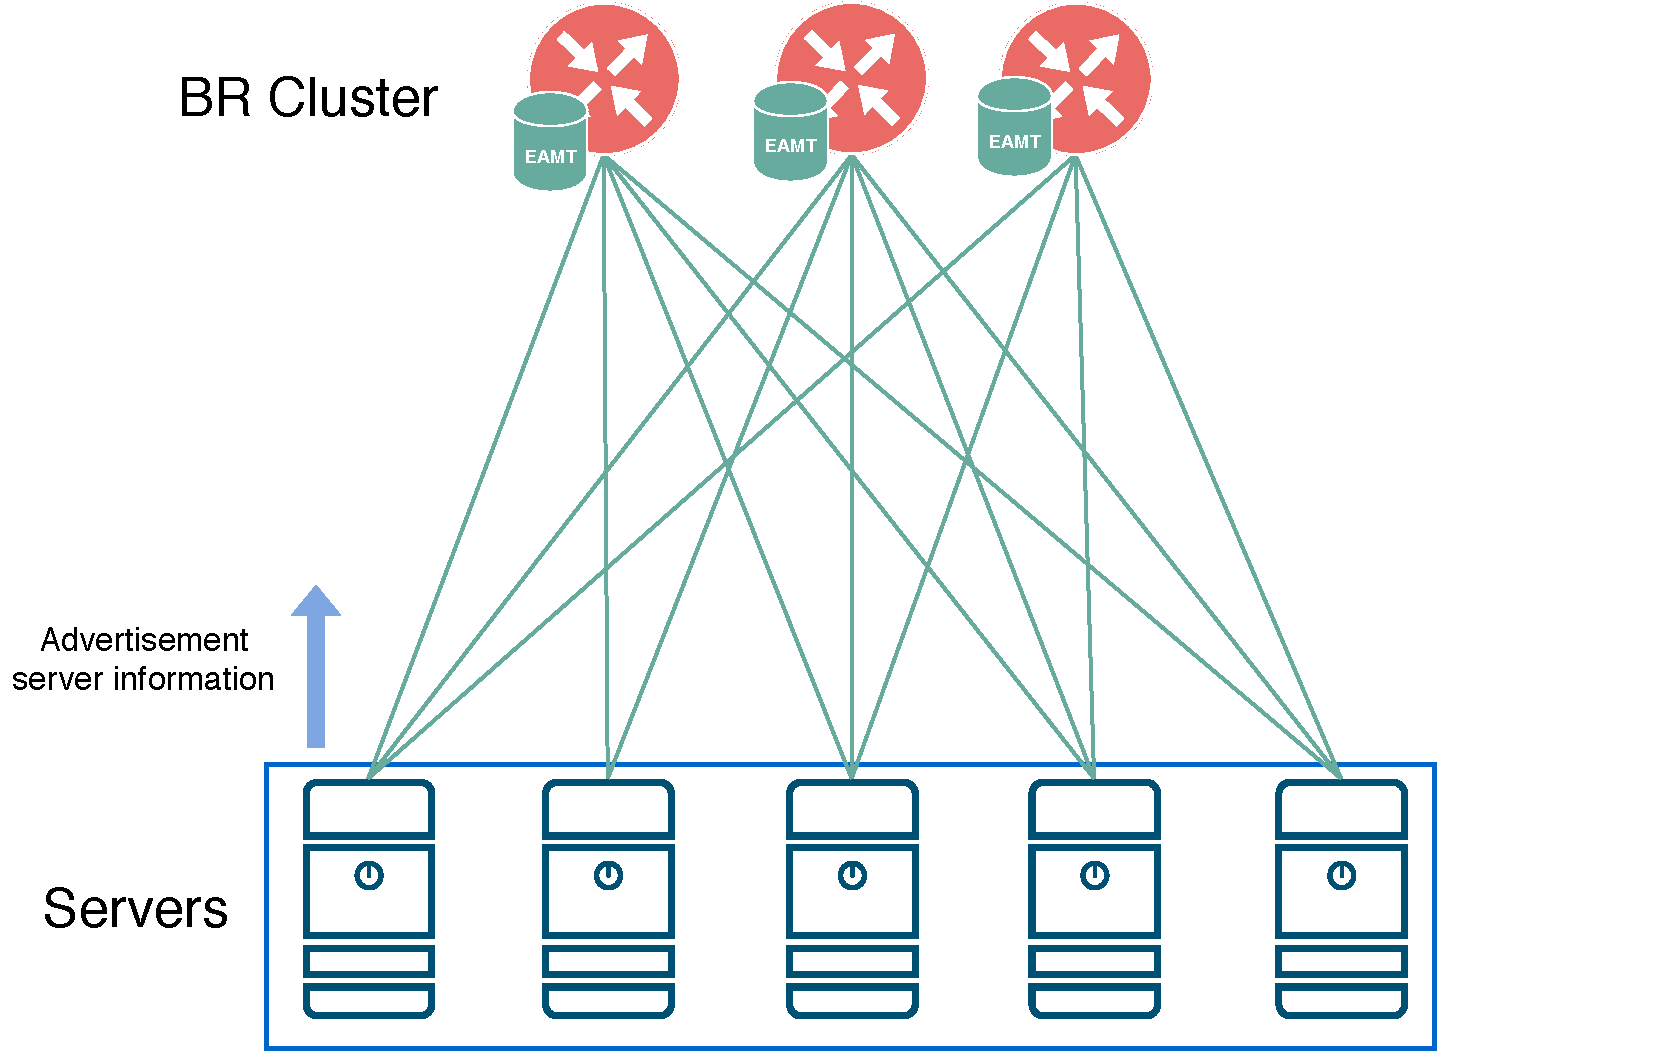
\includegraphics[width=12cm,pagebox=cropbox,clip]{img/approach_distributed_model.pdf}
    \end{center}
    \caption{分散管理型アプローチによるダイナミックEAMT}
    \label{fig:approach_distributed_model}
\end{figure}

\subsubsection{要件評価}

\begin{itemize}
    \item BR間のEAMTの一貫性 \\
    各BR間でEAMT一貫性を保証する機構は無いが,当該BRと疎通できないサーバーは障害時に自身のIPv4サービスアドレう宛のトラフィックを当該BRに経由させることが出来ないため,問題にならない.
    \item 変更追従性 \\
    サーバー自身のエージェントプロセスが直接BRに広告を行うため,実際の変更にリニアに対応出来る.
    \item スケーラビリティ \\
    EAMTの制御に必要とする通信コネクション数$C$は以下の通りになる.
    \begin{equation}
        C =  M \cdot N 
    \end{equation}
    サーバー群・各BR間でフルメッシュでのコネクションが必要なため,SIIT-DCネットワーク自体が小規模の場合のみ採用可能である.

    \item デプロイメントの容易さ \\
    各サーバー・BRにエージェントを導入する必要があるが,システム自体の機能は軽量である.
\end{itemize}

\section{アプローチの検討}

中央管理型アプローチが各BR間でのEAMT一貫性,スケーラビリティの二要素で優位であるが,コントローラーの役割が非常に大きくなり機能要件が高くなるため,変更追従性とデプロイメントの容易さの面での障壁が高いという問題も抱えている.一方で分散管理型アプローチはシンプルな構成であるためデプロイメントが比較的容易であり変更への追従がリニアであるが,各サーバーが通信コネクションを多量に貼らなくてはならない点でスケーラビリティに難がある.

本提案手法では両アプローチを総合した動的経路制御プロトコルであるiBGPを利用したハイブリッド型アプローチを提案する.第\ref{proposal}章において,本提案手法を中央管理型・分散型の両アプローチと比較する.


%%% Local Variables:
%%% mode: japanese-latex
%%% TeX-master: "../bthesis"
%%% End:

\chapter{本提案手法の設計}
\label{proposal}
第\ref{consideration}章では,DynamicEAMTを設計する上で考えられる二種類のアプローチについて,求められる要件に照らし合わせて評価・検討を行った.
本章では検討結果の得られた内容を基に,iBGPを利用したDynamicEAMTの実現手法の設計に関して論じる.


本章では提案手法の設計を述べる.

\section{概要}
分散管理と中央管理のいいところどりが可能な、iBGP + RR構成を取る


\section{BGP}
\subsection{概要}
用途

iBGPとEBGP

\subsection{特徴}
\subsubsection{マルチプロトコル}
\subsubsection{実装が一般的}
OSSもある
\subsubsection{軽量}

\subsection{iBGPとルートリフレクター}
\subsubsection{用途}
\subsubsection{Dynamic EAMTでのメリット}

\section{ネットワーク設計}
ネットワーク図を書く

\section{各ノードの役割と要件}
\subsection{BR}

\subsubsection{BGPデーモン}
\subsection{SIIT機構}
\subsection{EAMT制御機構}



\subsection{IPv4サービス提供サーバー}
\subsubsection{BGPデーモン}
\subsubsection{サービスアドレス広告機構}


\subsection{RR}
\subsubsection{BGPデーモン}
\subsubsection{ルートリフレクター機構}

\subsection{各アプローチとの比較}
星取り表を書く

%%% Local Variables:
%%% mode: japanese-latex
%%% TeX-master: "../bthesis"
%%% End:

\chapter{プロトコル設計と実装}
\label{implementation}
本章では,第\ref{proposal}章で述べた提案システムのメッセージ設計と実装について述べる.

\section{BGP UPDATEメッセージの設計}
本提案手法ではサーバー・BR・ルートリフレクター間のメッセージングにBGPを利用する.
本節ではBGP UPDATEメッセージの設計を行う.
\subsection{要件}
Dynamic EAMTを実現するにあたって,EAMとして広告すべきに必要な属性は1) IPv4サービスアドレス,2)IPv6サービスアドレス, 3)変換プレフィックスの3種が想定される.
表\ref{table:eam_required}に各属性の情報を列記する.

\begin{table}[h]
    \label{table:eam_required}
    \caption{EAMに必要な情報}
    \resizebox{\textwidth}{!}{%
    \begin{tabular}{cccc}
    \hline
    属性名 & 型 & 備考 & 例 \\ \hline
    IPv4 サービスアドレス & IPv4 ネットワークアドレス & IPv6サービスアドレスとホストアドレス長が一致 & 192.0.2.1/32 \\ \hline
    IPv6 サービスアドレス & IPv6 ネットワークアドレス & IPv4サービスアドレスとホストアドレス長が一致 & 2001:db8:200::1/128 \\ \hline
    変換プレフィックス & IPv6 ネットワークアドレス(/96) &  & 64:ff9b::/96 \\ \hline
    \end{tabular}%
    }
\end{table}

\subsection{実装}
本提案手法では,IPv6ユニキャスト経路\footnote{アドレスファミリー番号 2, サブアドレスファミリー番号 1\cite{IANA_AFI,IANA_SAFI}}として,BGPを利用してEAMを広告・交換する.
UPDATEメッセージ以外の扱いは標準的なBGPメッセージに準ずる.

\subsubsection{BGP UPDATEメッセージ}
本提案手法におけるBGP UPDATEメッセージに含有するパス属性\footnote{Path Attributes}を図\ref{table:bgp_eam}のように定義した.


\begin{table}[]
    \label{table:bgp_eam}
    \caption{BGP UPDATEメッセージにおける各パス属性}
    \resizebox{\textwidth}{!}{%
    \begin{tabular}{cllclc}
    \hline
    \begin{tabular}[c]{@{}c@{}}タイプ\\ コード値\end{tabular} & \multicolumn{1}{c}{パス属性} & 必須 & 値 & \multicolumn{1}{c}{備考} & 例 \\ \hline
    1 & ORIGIN & 必須 & 2(IMCOMPLETE) & 本実装においては利用しない. & 2 \\ \hline
    2 & AS\_PATH & 必須 & AS番号 & iBGPのみで広告するため,自身のAS番号を記載する & 65001 \\ \hline
    5 & LOCAL\_PREF & \multicolumn{1}{c}{任意} & 1 $\sim$65535 & EAMの優先度 & 200 \\ \hline
    8 & COMMUNITY & \multicolumn{1}{c}{任意} & {[}0$\sim$65535{]}:{[}0$\sim$65535{]} & BGP コミュニティ名 & 2500:200 \\ \hline
    9 & ORIGINATOR\_ID & 必須 & \multicolumn{1}{l}{BGP Identifier} & 自身のルーターID & 192.0.2.1 \\ \hline
    10 & CLUSTER\_LIST & 任意 & \multicolumn{1}{l}{クラスターID} & \begin{tabular}[c]{@{}l@{}}ルートリフレクターを利用する場合,要指定\\ 同じEAMTを共有する範囲を指定する\end{tabular} & 192.0.2.1 \\ \hline
    14 & \begin{tabular}[c]{@{}l@{}}MP\_REACH\_NLRI\\ -\textgreater NLRI\end{tabular} & \multicolumn{1}{c}{必須} & IPv6アドレス+プレフィックス長 & 変換プレフィックス + IPv4サービスアドレス/128 & 64:ff9b::192.0.2.1/128 \\ \hline
    14 & \begin{tabular}[c]{@{}l@{}}MP\_REACH\_NLRI\\ -\textgreater NEXT\_HOP\end{tabular} & 必須 & IPv6アドレス & 変換プレフィックス + IPv4サービスアドレス/128 & 2001:db8:200::1 \\ \hline
    15 & MP\_UNREACH\_NLRI & \multicolumn{1}{c}{必須} & \multicolumn{3}{c}{MP\_REACH\_NLRIと同様} \\ \hline
    \end{tabular}%
    }
\end{table}

\subsection{実装時に留意すべき事項}
BGPを利用したDynamic EAMTにおいて留意すべき事項を述べる.
\subsubsection{ルーティングテーブルの隔離}
通常のIGP・EGP経路とは用途が異なるため,何らかの仮想化技術を利用してそれらとEAMTをBGPスピーカーが区別する必要がある.
具体的にはVRF\footnote{Virtual routing and forwarding}などのルーティングテーブル仮想化技術の利用が想定される.

\subsubsection{ホストルートでの利用に限定}
本提案手法ではMP\_REACH\_NLRI及びMP\_REACH\_NLRIのアドレスファミリーとしてIPv6ユニキャスト経路を利用している.そのため実装上の問題から,IPv6サービスアドレス及びIPv4サービスアドレスがそれぞれ1アドレスの場合のみをサポートしている.


\section{PoCの実装}
\label{implementation:poc}
第\ref{evaluation}章で行う概念検証実験にもちいるPoC\footnote{Proof of Concept. 概念検証実装}について,各ノードで必要なコンポーネントとその役割及び具体的な実装について記述する.


\subsection{各コンポーネントの実装}
\label{implementation:poc:components}

\begin{figure}[h]
    \begin{center}
    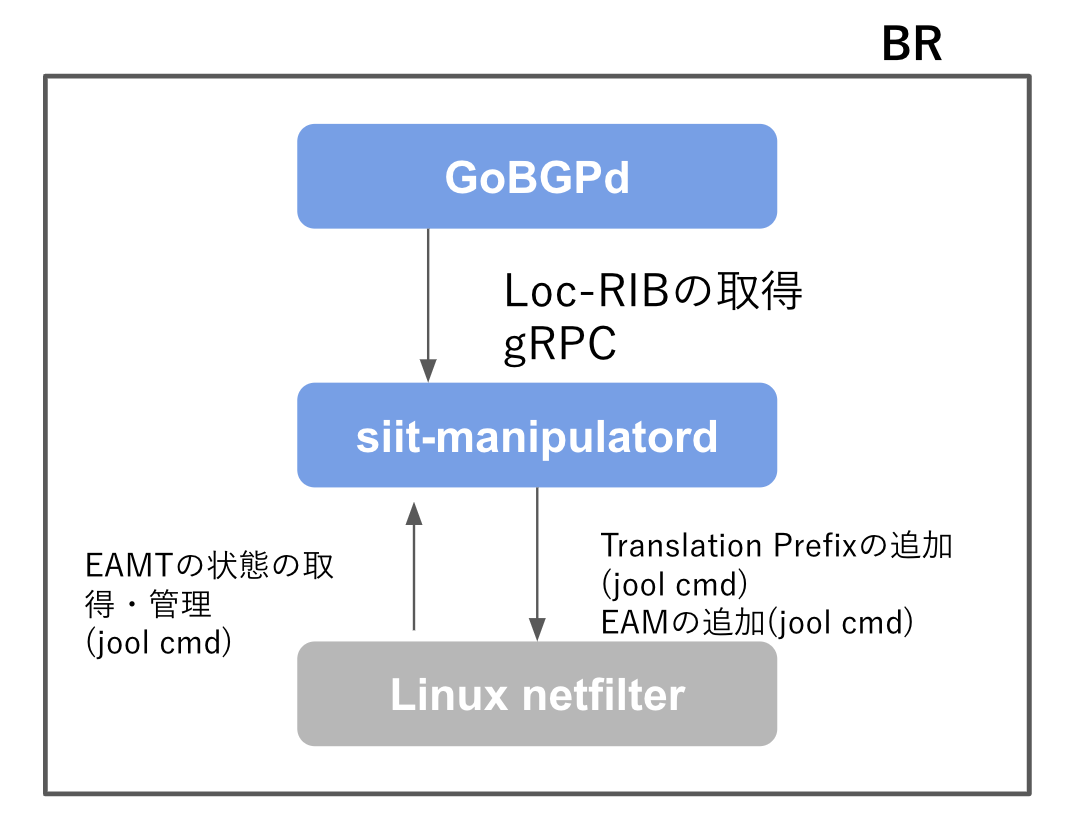
\includegraphics[width=12cm,pagebox=cropbox,clip]{img/poc_implementation.png}
    \end{center}
    \caption{BRに必要なコンポーネント群の関係図}
    \label{fig:poc_implementation}
\end{figure}

第\ref{proposal:network:nodes}項で述べたコンポーネント群は以下の様にそれぞれ実装した.
BRにおけるBRに必要なコンポーネント群の関係図を図\ref{fig:poc_implementation}に示す.表refにコンポーネント群の情報の概要を示す.


\subsubsection{BGPデーモン}
BGPデーモンには,OSSのBGPデーモンであるGoBGP\footnote{\url{https://osrg.github.io/gobgp/}}を利用する.

GoBGPではgRPC\footnote{gRPC Remote Procedure Calls. \url{https://www.grpc.io/}}を用いた操作機構が実装されており,同期・非同期を問わず他のアプリケーションとの連携が容易に行える.
RouteReflector機構もサポートされているため,本PoCでは全てのノードのBGPデーモンとしてこれを利用する.

\subsubsection{SIIT}
SIITにはJool\footnote{Jool. \url{https://jool.mx/en/index.html}}のSIIT モードを利用する.

JoolはLinuxOSで利用できるNAT64/SIIT環境で,Lunux Netfilterによって実装されており,汎用的に様々なプラットフォームでの利用が可能である\cite{JOOL,quintero2016performance}.
EAMTの変更には専用のCLIコマンドを利用する.

\subsubsection{EAMT制御機構}
\label{implementation:poc:siit-manipulatord}
BGP上で受信したLoc-RIBをEAMTに反映するために,EAMT制御機構"siit-manipulatord"を実装した.
gRPCによってGoBGPのLoc-RIBの変化を監視し,JoolのCLIコマンドを利用してLinux NetFilterに変更を反映するほか,Translation Prefixの定義などSIITに必要な情報を管理する.

\subsection{メッセージングと状態遷移}
\label{implementation:poc:sequence}

\begin{figure}[h]
    \begin{center}
    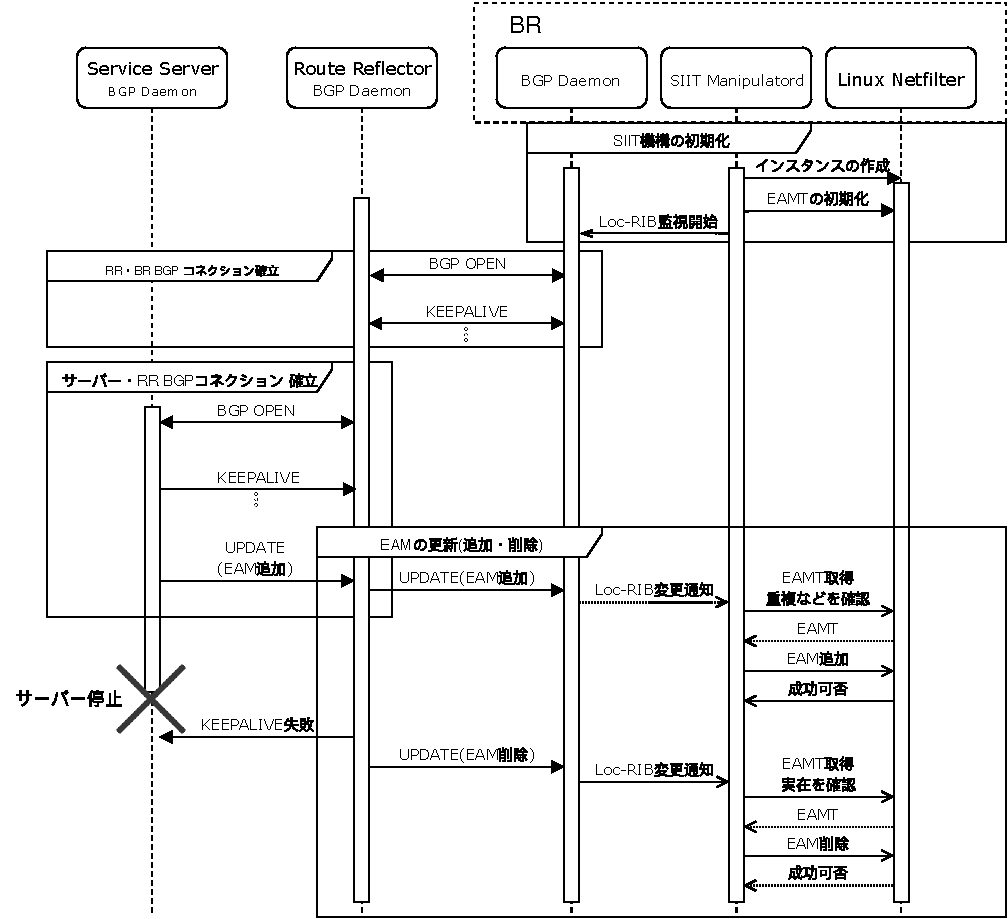
\includegraphics[width=15cm,pagebox=cropbox,clip]{img/sequence_manipulatord.pdf}
    \end{center}
    \caption{本PoCにおける各ホスト・コンポーネントの相互作用と状態遷移}
    \label{fig:poc_implementation}
\end{figure}

図\ref{fig:poc_implementation}にIPv4サービス提供サーバー・ルートリフレクター・BRの相互作用と状態遷移の概要を示す.

以下に各状態にあるホスト・コンポーネント間の相互作用に関して記述する.

\subsection{SIIT機構の初期化}
BRは起動後ネットワーク環境の準備が出来次第,BGPデーモンとSIIT制御機構のサービスを開始する.EAMT制御機構は初めにLinux Netfilterを操作し,SIITによるプロトコル変換を行うインスタンス\footnote{Jool Instance. ネットワーク名前空間ごとに一つ存在可能である.以後変換インスタンスと呼称する.}を作成する.このインスタンスはBRが利用する変換プレフィックスを保持する.その後EAMTを初期化し,gRPCを利用してBGPデーモンからLoc-RIBの監視を開始する.以後Loc-RIBに変更があるまで待機する.Loc-RIBの変更はベストパスの変更に伴っても発生するため,BGP NOTIFICATIONメッセージなどにより,ベストパスとなる経路情報を発信していたBGPピアとのコネクションが切断されたような場合にも,SIIT制御機構に変更通知が送信される.


\subsection{ルートリフレクター・BR間のBGPコネクションの確立と維持}
BRのBGPデーモンは起動次第,事前に登録されたルートリフレクターに対するBGP OPENメッセージの送信を開始し,BGPコネクションの確立を試みる.
RRからのBGP OPENメッセージの回答を受けてBGPコネクションを確立し,以後BGP KEEPALIVEメッセージによって接続性の死活監視を行う.



\subsection{IPv4サービス提供サーバー・ルートリフレクター間のBGPコネクションの確立と維持}
IPv4サービス提供サーバーのBGPデーモンは起動に伴って,自身のLoc-RIBにEAM(変換プレフィックスとIPv4サービスアドレスによって構成されたNLRIを埋め込んだ経路情報)を登録する.
BGPコネクションが確立次第,IPv4サービス提供サーバーはUPDATEメッセージによりEAMの追加をルートリフレクターに通知する.
このコネクションでも同様に,以後BGP KEEPALIVEメッセージによって接続性の死活監視を行う.


\subsection{EAMの追加}
IPv4サービス提供サーバーからUPDATEメッセージはルートリフレクターにより各BRに伝達され,UPDATEメッセージを受信したBRのBGPデーモンは自身のLoc-RIBを更新する.

Loc-RIBの更新に伴いLoc-RIBの監視を行っていたSIIT制御機構にgRPCを介し更新通知が送信される.以後のSIIT制御機構の処理はコルーチンを利用した非同期処理によって行われるため,EAMT走査にまつわる処理を行っている最中であってもLoc-RIBの監視はブロッキングされない.

SIIT制御機構はEAMTの更新を滞りなく行うため,LinuxNetfilterに登録された現在のEAMTの状態を取得し,競合するEAMが登録されていないことを確認する.IPv4サービスアドレスとIPv6サービスアドレスが一致するEAMが存在していた場合や事前に登録された変換プレフィックスに一致しない場合,以後の処理をスキップする.

新しく受信したEAMに問題がない場合,SIIT制御機構はEAMの追加を試みる.Linux Nefilterは新しいEAMが追加されたEAMTを参照し,直ちにパケットのフォワーディングを開始する.

\subsection{EAMの削除}
ルートリフレクターは,何らかの理由でIPv4サービス提供サーバーとのBGP KEEPALIVEメッセージが失敗した場合やBGP NOTIFICATIONメッセージを受信した場合,自身のLoc-RIBから該当のEAMを削除し,Adj-RIB-OUTの情報を更新する.

ルートリフレクターからEAM削除を広告するBGP UPDATEメッセージを受け取ったBRのBGPデーモンはLoc-RIBを更新し,SIIT制御機構に対してLoc-RIB変更通知を送信する.EAMの追加時と同様に,EAMTを取得して該当するEAMの実在を確認後,SIIT制御機構はEAM削除を試みる.

\subsection{EAMの更新}
BGP経路情報の属性値の変更などに伴ってBRのLoc-RIBに登録されるベストパスが変更になる場合がある.

BRのBGPデーモンはEAM追加・削除時同様に,SIIT制御機構に対してLoc-RIB変更通知を送信する.この変更通知に伴ってEAMT上の古いEAMは削除され,新しいEAMに更新される.




%%% Local Variables:
%%% mode: japanese-latex
%%% TeX-master: "./thesis"
%%% End:

\chapter{評価}
\label{evaluation}
本章では,第\ref{proposal}章及び第\ref{implementation}章で設計・実装に関して述べた本提案手法に関して,第\ref{issue:siit-dc_problems}節で指摘したSIIT-DCの課題に対して有効性があることを評価する.



\section{評価要件}
\label{evaluation:requirements}
SIIT-DCにおけるダイナミックEAMT機構では,第\ref{consideration:points}節で述べた事項が求められる.
それらを定量的に評価するための指標・尺度について記述する.


\subsection{BR間のEAMTの一貫性}
\label{evaluation:requirements:consistency}

SIIT-DCネットワークにおける各BRは一貫性のあるEAMTを保持する必要がある.
本評価実験では後に述べるテストケースにおいて,以下の2点を検証することで各BRのEAMTが一貫性を有すると定義する.
\begin{itemize}
    \item \textbf{EAM数の収束} \\
    EAMの更新が行われる事象が発生した場合に,一定の収束時間が経過した後に各BRのEAMTのレコード数が変化することなく,一意に収束すること.
    \item \textbf{EAMTのレコードの内容} \\
    EAM数が収束した際に各BRの有するEAMTの内容に差異が無いこと.
\end{itemize}

\subsection{変更追従性}
\label{evaluation:requirements:change}
前に述べたように,従来のSIIT-DCの構成では,IPv4サービスが追加・削除・変更された場合やBRの追加配備を行った場合に,各BRのEAMTの内容を適宜変更する必要があった.

本研究ではEAMT変更が必要な事象が発生した場合に,運用者が特別なオペレーションを行うことなくサービス提供を想定通りに開始・継続・中断される状況を,EAMTが変更に追従している状態であると定義する.

本評価実験では下記の様なEAMT変更が必要な事象を想定する.

\begin{itemize}
    \item \textbf{IPv4サービスの追加・削除} \\
    ネットワーク内のIPv6サービスにおいて,IPv4サービスアドレスを付与することでIPv4/IPv6の両プロトコルによるサービス提供を開始する場合.もしくは,そのサーバが行っているIPv4サービス提供を中断する場合.
    \item \textbf{IPv4サービス提供サーバの変更} \\
    SIIT-DCにおいて提供中のIPv4サービスに関して,他のIPv6アドレスを持つサーバによるサービス提供を改めて開始する場合.
    \item \textbf{BRの追加・撤去} \\ 
    対外接続点に新しいBRを追加もしくは稼働中のBRを撤去しながらIPv4サービスを継続して行う場合.
\end{itemize}

% AWSのElastic LoadbalancerのTimeout時間は5秒. 1サービスアドレうあたり5秒以内に収束したら良いのでは.

\subsection{スケーラビリティ}
\label{evaluation:requirements:scalability}
ダイナミックEAMTを実現する機構は対外接続点やIPv4提供サービスの増加に柔軟に対応可能であることが望ましい.

本評価実験では各ノードのスケールにおいては下記を想定した評価試験用ネットワークを実装する.
IPv4提供サービスの総数が増加した場合においても,本提案手法が動作が可能であることを評価する.

\begin{itemize}
    \item BR: 30ホスト 
    \item ルートリフレクタ: 2ホスト 
    \item IPv4提供サーバ: 10 〜 1000ホスト
\end{itemize}


\section{実験環境}
\label{evaluation:environment}

本評価実験で利用した実験環境について述べる.

\subsection{ネットワークトポロジ}
\begin{figure}[H]
    \begin{center}
    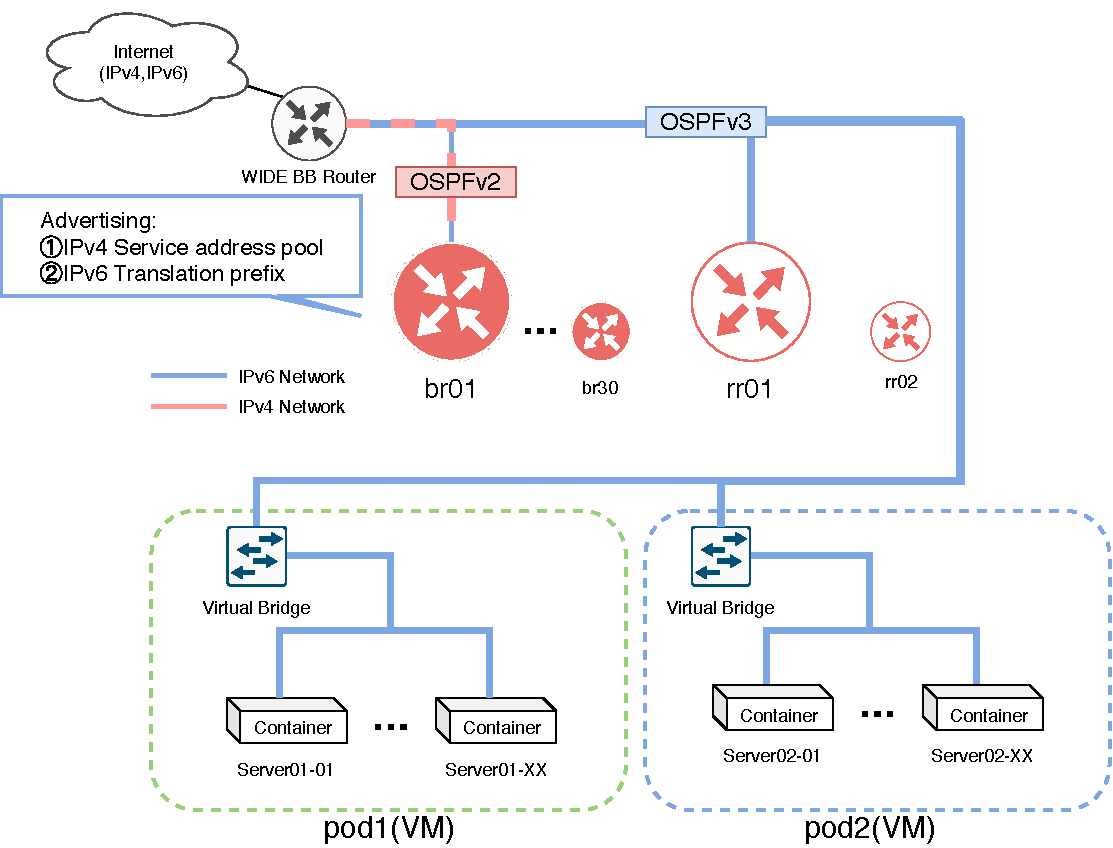
\includegraphics[width=15cm,pagebox=cropbox,clip]{img/evaluation_experiment_no_injector.pdf}
    \end{center}
    \caption{評価実験におけるネットワークと各ホスト}
    \label{fig:evaluation_experiment}
\end{figure}

本評価実験を行うために,WIDEプロジェクト\footnote{\url{https://www.wide.ad.jp/}}藤沢NOC内に実験用ネットワークを構築した.図\ref{fig:evaluation_experiment}は本実験用ネットワークの概略を示す.
本ネットワークでは第\ref{issue:siit-dc-merit:scalability}項で述べたECMPエニーキャストによるBRの水平スケールを可能にするネットワークトポロジを採用している.


本ネットワークでは,BR群(br01 $\cdots$ br30)のみWIDEネットワークを介してIPv4インターネットに接続している.WIDEプロジェクト内のルータに対して,IPv4サービス提供サーバ群(Server01-01  $\cdots$ Server02-60)が利用するIPv4サービスアドレス群を,OSPFv2\cite{RFC2328}を利用したECMPエニーキャストにて広告する.これにより,インターネット上のIPv4クライアントからのIPv4パケットはいずれかのBRを経由し,ダイナミックEAMTを参照したSIITによるネットワークプロトコル変換が各BRにて行われたのち,IPv6パケットとして各IPv4サービス提供サーバに転送される.

各ホストは共通のIPv6ネットワーク上に所属し,WIDEプネットワークを介したインターネット疎通性を持つ.このIPv6ネットワークでは,各BRからIPv4サービス提供サーバ向けに,OSPFv3\cite{RFC5340}を利用したECMPエニーキャストによる変換プレフィックス向け経路広告が行われている.IPv4サービス提供サーバからの変換プレフィックス宛のパケットは,いずれかのBRを経由してSIITによるネットワークプロトコル変換がなされたあと,インターネット上のIPv4提供クライアントに向けて返送される.

各ホスト間のダイナミックEAMTに用いるBGPメッセージングは各ホストが共通して属するIPv6ネットワークを介して行われる.BR群及びIPv4サービス提供サーバ群はルートリフレクタ群(rr01 $\cdots$ rr02)に対して,IPv6によるIBGPコネクションを確立する.本ネットワークではルートリフレクタ間のBGPメッセージングは行わない一層のルートリフレクタ構成を採用する.各IPv4サービス提供サーバからの経路情報はネットワーク内で一意のクラスタIDを付与した上でBR群に広告される.

なお,本実験環境ではBGPコネクションを維持するための各種パラメータを表\ref{table:eval_bgp_timer}の様に指定する.

各ホストは各BRはNTP(Network Time Protocol)\cite{RFC5905}を利用した時刻同期を行う.同一ネットワーク上のNTPサーバを参照元とし,十分な精度で同期を行えていると仮定する.


\begin{table}[]
    \label{table:eval_bgp_timer}
    \caption{BGPコネクションで利用したパラメータ}
    \centering
    \resizebox{\textwidth}{!}{%
    \begin{tabular}{lcl}
    \hline
    \multicolumn{1}{c}{要素} & 値 & \multicolumn{1}{c}{説明} \\ \hline
    Keep Alive Interval & 3秒 (標準:60秒) & KEEPALIVEメッセージの送信間隔 \\
    Hold Time & 9秒 (標準:180秒) & この値以上KEEPALIVEの到達を確認出来なかった場合,当該ピアから受信した経路を破棄する. \\
    ConnectTimer & 5秒 (標準:120秒) & BGPコネクションの再試行を行う間隔. \\ \hline
    \end{tabular}%
    }
\end{table}

\subsection{実装}
本項では各ホストの実行環境について記述する.
各ホストが利用している,BGPデーモン・SIIT機構・EAMT制御機構の各コンポーネントは第\ref{implementation:poc:components}項で述べたPoCと同一の物を利用している.


\subsubsection{BR}
本評価ネットワークにおけるBR群は,同一物理サーバで仮想マシンとして稼働する.
図\ref{table:eval_env_BR}に物理サーバと仮想マシンの実行環境を詳細に示す.

また本実験では,現在保有しているEAMT数・BGP経路数を計測するための監視プロセスを0.2秒毎に実行し,各種評価要件の検証に利用する.

\begin{table}[h]
    \label{table:eval_env_BR}
    \caption{評価実験用BR群の実行環境}
    \resizebox{\textwidth}{!}{%
    \begin{tabular}{|cccc}
    \hline
    \multicolumn{4}{|c|}{\cellcolor[HTML]{EFEFEF}\textbf{計算環境}} \\ \hline
    \multicolumn{1}{|c|}{機種} & \multicolumn{1}{c|}{CPU} & \multicolumn{1}{c|}{RAM} & \multicolumn{1}{c|}{NIC} \\ \hline
    Intel S2600WTT & 2CPU: Intel Xeon E5-2699 v3 2.30GHz & 64GB & \multicolumn{1}{c|}{Intel 82599EB 10-Gigabit SFI/SFP+} \\ \hline
    \multicolumn{4}{|c|}{\cellcolor[HTML]{EFEFEF}\textbf{ハイパーバイザ環境}} \\ \hline
    \multicolumn{1}{|c|}{OS} & \multicolumn{1}{c|}{バージョン} & \multicolumn{1}{c|}{vCPU} & \multicolumn{1}{c|}{備考} \\ \hline
    VMware ESXi & 6.7.0 & 72 & \multicolumn{1}{l|}{build: 5160138} \\ \hline
    \multicolumn{4}{|c|}{\cellcolor[HTML]{EFEFEF}\textbf{仮想マシン}} \\ \hline
    \multicolumn{1}{|c|}{OS} & \multicolumn{1}{c|}{カーネル} & \multicolumn{1}{c|}{リソース} & \multicolumn{1}{c|}{利用コンポーネント} \\ \hline
    Ubuntu 18.04.3 LTS & 4.15.0-72-generic & vCPU: 2 RAM:2GB & \multicolumn{1}{l|}{BGPデーモン,EAMT制御機構,SIIT機構} \\ \hline
    \end{tabular}%
    }
\end{table}





\subsubsection{ルートリフレクタ}
本評価ネットワークにおけるBR群は,同一物理サーバで仮想マシンとして稼働する.
図\ref{table:eval_env_RR}に物理サーバと仮想マシンの実行環境を詳細に示す.

ルートリフレクタではGoBGPにてルートリフレクタ機能に加えてダイナミックネイバー機能を有効化する.通常,BGPコネクションを確立するためにはBGPピア間で互いのピアリングアドレスを明示的に設定する必要があるが,本機能を利用することで動的に多数のBGPスピーカとのピアリングが可能になる\cite{GoBGP_dynamic}.同様の機構は他のBGPデーモン・ネットワーク機器でも実装されている\cite{Cisco_dynamic}.


\begin{table}[]
    \label{table:eval_env_RR}
    \caption{評価実験用RR群の実行環境}
    \resizebox{\textwidth}{!}{%
    \begin{tabular}{|cccc}
    \hline
    \multicolumn{4}{|c|}{\cellcolor[HTML]{EFEFEF}\textbf{計算環境}} \\ \hline
    \multicolumn{1}{|c|}{機種} & \multicolumn{1}{c|}{CPU} & \multicolumn{1}{c|}{RAM} & \multicolumn{1}{c|}{NIC} \\ \hline
    Dell PowerEdge R410 & 2CPU: Intel Xeon E5530 @ 2.40GHz & 16GB & \multicolumn{1}{c|}{HP NC522SFP Dual Port 10GbE Server Adapter} \\ \hline
    \multicolumn{4}{|c|}{\cellcolor[HTML]{EFEFEF}\textbf{ハイパーバイザ環境}} \\ \hline
    \multicolumn{1}{|c|}{OS} & \multicolumn{1}{c|}{バージョン} & \multicolumn{1}{c|}{vCPU} & \multicolumn{1}{c|}{備考} \\ \hline
    VMware ESXi & 6.5.0 & 16 & \multicolumn{1}{l|}{build: 15256549.} \\ \hline
    \multicolumn{4}{|c|}{\cellcolor[HTML]{EFEFEF}\textbf{仮想マシン}} \\ \hline
    \multicolumn{1}{|c|}{OS} & \multicolumn{1}{c|}{カーネル} & \multicolumn{1}{c|}{リソース} & \multicolumn{1}{c|}{利用コンポーネント} \\ \hline
    Ubuntu 18.04.3 LTS & 4.15.0-72-generic & vCPU: 4 RAM:4GB & \multicolumn{1}{l|}{BGPデーモン} \\ \hline
    \end{tabular}%
    }
\end{table}

\subsubsection{IPv4サービス提供サーバ}
本実験環境において,IPv4サービス提供サーバ群はコンテナ型仮想化\cite{soltesz2007container}を利用し,二つのホスト仮想マシン上で実行される.
図\ref{table:eval_env_server}に物理サーバとホスト仮想マシン及びコンテナの実行環境を詳細に示す.


\begin{table}[h]
    \label{table:eval_env_server}
    \caption{評価実験用IPv4サービス提供サーバ群の実行環境}
    \resizebox{\textwidth}{!}{%
    \begin{tabular}{|cccc}
    \hline
    \multicolumn{4}{|c|}{\cellcolor[HTML]{EFEFEF}\textbf{計算環境}} \\ \hline
    \multicolumn{1}{|c|}{機種} & \multicolumn{1}{c|}{CPU} & \multicolumn{1}{c|}{RAM} & \multicolumn{1}{c|}{NIC} \\ \hline
    Dell PowerEdge R410 & 2CPU: Intel Xeon E5530 @ 2.40GHz & 48GB & \multicolumn{1}{c|}{HP NC522SFP Dual Port 10GbE Server Adapter} \\
    \multicolumn{1}{|l}{Dell PowerEdge R410} & \multicolumn{1}{l}{2CPU: Intel Xeon E5530 @ 2.40GHz} & 48GB & \multicolumn{1}{l|}{HP NC522SFP Dual Port 10GbE Server Adapter} \\ \hline
    \multicolumn{4}{|c|}{\cellcolor[HTML]{EFEFEF}\textbf{ハイパーバイザ環境}} \\ \hline
    \multicolumn{1}{|c|}{OS} & \multicolumn{1}{c|}{バージョン} & \multicolumn{1}{c|}{vCPU} & \multicolumn{1}{c|}{備考} \\ \hline
    VMware ESXi & 6.5.0 & 16 & \multicolumn{1}{l|}{build: 15256549. Pod1,Pod2で共通} \\ \hline
    \multicolumn{4}{|c|}{\cellcolor[HTML]{EFEFEF}\textbf{ホスト仮想マシン}} \\ \hline
    \multicolumn{1}{|c|}{OS} & \multicolumn{1}{c|}{カーネル} & \multicolumn{1}{c|}{リソース} & \multicolumn{1}{c|}{備考} \\ \hline
    Ubuntu 18.04.3 LTS & 4.15.0-72-generic & vCPU: 4 RAM:4GB & \multicolumn{1}{l|}{Pod1, Pod2で共通} \\ \hline
    \multicolumn{4}{|c|}{\cellcolor[HTML]{EFEFEF}\textbf{コンテナ}} \\ \hline
    \multicolumn{1}{|c|}{OS} & \multicolumn{1}{c|}{コンテナエンジン} & \multicolumn{1}{c|}{コンテナイメージ} & \multicolumn{1}{c|}{利用コンポーネント} \\ \hline
    Alpine Linux 3.11 & Dockerversion 19.03.5 & 自作 & \multicolumn{1}{l|}{GoBGPデーモン} \\ \hline
    \end{tabular}%
    }
\end{table}


\section{評価実験1: EAMTの収束・一貫性の検証}
\label{evaluation:eval1}

本節では\ref{evaluation:requirements}項で述べた3要件のうち,「BR間のEAMTの一貫性」及び「スケーラビリティ」の検証を目的とした評価実験を行い,その詳細と結果について記述する.

\subsection{シナリオ}
基本的なSIIT-DCネットワークの構築を想定し,IPv4提供サービスサーバー群を起動した後に,BR間のEAMTの一貫性が正しく担保されるかを検証する.

\subsubsection{手順}
以下のような手順を1単位として,IPv4サービス提供サーバ数$x$につき各1回試行する.
\begin{enumerate}
    \item \textbf{ルートリフレクタの起動} \\
    ルートリフレクタ群を起動し,BGPデーモンの立ち上げを確認する.
    \item \textbf{BRの起動} \\
    BRを起動し,BGPデーモン・EAMT制御機構の立ち上げを確認する.
    \item \textbf{IPv4サービス提供サーバの起動} \\
    IPv4サービス提供サーバを$x$ホスト起動し,それぞれのサーバにおいてBGPデーモンの立ち上げ及びEAMのLoc-RIBへの反映を確認する.この時利用するIPv4サービスアドレスは事前に作成した正答となるEAMTを参照する.実験環境の都合上,サーバの起動は同期的に行う.
    \item \textbf{計測} \\
    全てのサーバが起動の起動を確認し,30秒後の各BRのEAMTの状態を収集する.EAMTの内容を事前に作成した正答と比較する.
\end{enumerate}

\subsection{説明変数・目的変数}
本実験環境におけるBRの数を$B$,事前に作成したEAMTに正答したBRの数$B_s$とし,正答率$R$を目的変数とする
目的変数$R$は以下の様な式\ref{eq:eval1}で表す事ができる.またIPv4サービス提供サーバの数を$x$とし,本評価実験の説明変数とする.

\begin{equation}
    R = \frac{B_s}{B}
    \label{eq:eval1}
\end{equation}


\subsection{条件}
各ホストの情報を表\ref{table:eval1_condition}に示す.記載の無いその他の条件は\ref{evaluation:environment}項に準ずる.

\begin{table}[]
    \label{table:eval1_condition}
    \caption{評価実験1での各ホストの情報}
    \resizebox{\textwidth}{!}{%
    \begin{tabular}{lcl}
    \hline
    \multicolumn{1}{c}{要素} & ホスト数 & ホスト名 \\ \hline
    BR & 30 & br01〜br30 \\
    ルートリフレクタ & 2 & rr01〜rr02 \\
    IPv4サービス提供サーバ & 10,100,200,400,500,600,700,800,900,1000& server01-01 〜 server01-500, server02-01 〜 server02-500 \\ \hline
    \end{tabular}%
    }
\end{table}


\subsection{結果}
\label{evaluation:eval1:result}
本評価実験の結果を表\ref{table:eval1_result}に示す.
IPv4提供サービスサーバ数$x$が600までの場合に,全てのBR間で保有するEAMTが収束し,一貫性を維持していることが読み取れる.
一方で$x>=700$の場合には全てのBRが正答に一致しておらず,且つ収束しないことがわかった.


\begin{table}[]
    \label{table:eval1_result}
    \caption{評価実験1での各ホストの情報}
    \centering
    \resizebox{\textwidth}{!}{%
    \begin{tabular}{lcl}
    \hline
    \multicolumn{1}{c}{$x$: IPv4サービス提供サーバの数} & $R$: 正答にEAMTが一致したBR数の割合 & EAMTの収束可否 \\ \hline
    10 & 100 \% & 収束 \\
    100 & 100 \% & 収束 \\
    200 & 100 \% & 収束 \\
    300 & 100 \% & 収束 \\
    400 & 100 \% & 収束 \\
    500 & 100 \% & 収束 \\
    600 & 100 \% & 収束 \\
    700 & 0 \% & 収束せず \\
    800 & 0 \% & 収束せず \\
    900 & 0 \% & 収束せず \\
    1000 & 0 \% & 収束せず \\ \hline
    \end{tabular}%
    }
\end{table}


\begin{minipage}{\textwidth}
    \begin{lstlisting}[caption=EAMTが収束しない時点のルートリフレクタのログの抜粋,label=code:experiment1_rr]
        Jan 06 13:11:56 rr01 gobgpd[18970]: {"Code":4,"Data":null,"Key":"2001:200:0:8831:1:0:6440:243","Subcode":0,"Topic":"Peer","level":"warning","msg":"received notification","time":"2020-01-06T13:11:56+09:00"}
        Jan 06 13:11:56 rr01 gobgpd[18970]: {"Key":"2001:200:0:8831:1:0:6440:243","Reason":"notification-received code 4(hold timer expired) subcode 0(undefined)","State":"BGP_FSM_ESTABLISHED","Topic":"Peer","level":"info","msg":"Peer Down","time
        Jan 06 13:12:00 rr01 gobgpd[18970]: {"Key":"2001:200:0:8831:1:0:6440:1d","State":"BGP_FSM_ESTABLISHED","Topic":"Peer","level":"warning","msg":"Closed an accepted connection","time":"2020-01-06T13:12:00+09:00"}
    \end{lstlisting}
\end{minipage}
    
    
当該期間中のルートリフレクタ(rr01)のログの抜粋をコード\ref{code:experiment1_rr}に示す.BGPピア(IPv4サービス提供サーバ)より,ルートリフレクタから送信されるBGP KEEPALIVEメッセージに問題がある旨を表すBGP NOTIFICATIONメッセージを受信していることがわかる.$x=700$の実験期間中,常にこのようなログが高頻度で観測されていた.すなわち,本問題はルートリフレクタが一定以上のBGPピアを収容する場合,正常にKEEPALIVEメッセージを送信出来ず,全体のBGPコネクションの維持に問題が生じることがわかる.







\section{評価実験2: 構成変更追従性の検証}
\label{evaluation:eval2}
本節では\ref{evaluation:requirements}項で述べた3要件のうち,「変更追従性」「スケーラビリティ」の検証を目的とした評価実験を行い,その詳細と結果について記述する.



\subsection{シナリオ}
IDCネットワークにおいてIPv4サービス構成が変更になったことを想定し,各BRのEAMTの収束までの時間を計測する.

\subsubsection{構成変更の定義}
\label{evaluation:eval2:scenario:definication}
本評価実験では以下の二つの事例をIPv4サービス提供サーバの構成変更等と定義する.

\begin{enumerate}
    \item IPv4サービス提供サーバの追加 \\
    IPv4サービス提供サーバ1台を新規に起動し,BGPデーモンの立ち上げ及び当該サーバ用のEAMのLoc-RIBへの反映を行う. 
    \item IPv4サービス提供サーバの削除 \\
    任意のIPv4サービス提供サーバ宛のパケットをコンテナホスト仮想マシン上でフィルターし,当該サーバがルートリフレクタと疎通不能な状態を再現する.
\end{enumerate}


\subsubsection{手順}
以下のような手順を1単位として,初期状態のIPv4サービス提供サーバ数$x$につき各30回試行する.
\begin{enumerate}
    \item \textbf{初期状態の準備} \\
    \ref{evaluation:eval1}節で行った,IPv4サービス提供サーバ$x$ホストが,各BRを介したIPv4サービスが提供可能になった状態を初期状態とする.
    \item \textbf{IPv4サービス提供サーバの構成変更} \\
    \ref{evaluation:eval2:scenario:definication}項で述べた二つの事例のうち,一つを実行する.
    \item \textbf{計測} \\
    IPv4サービス提供サーバの構成変更から,各BRのEAMTが収束\footnote{ここでは\ref{evaluation:requirements:consistency}項で述べたEAMTが一貫性を維持した状態とする.}するまでに経過した時間を計測する.
\end{enumerate}

\subsection{説明変数・目的変数}
\label{evaluation:eval2:scenario:vars}

第\ref{implementation:poc:sequence}項で述べたように,BRのEAMTがIPv4サービス提供サーバの追加に追従するまでに必要な各コンポーネントの動作を以下の5つ分類することが出来る.
\begin{enumerate}
    \item IPv4サービス提供サーバがLoc-RIBにEAMを反映
    \item IPv4サービス提供サーバとルートリフレクタ間のBGPコネクションの確立
    \item IPv4サービス提供からBGP UPDATEメッセージがルートリフレクタに伝達
    \item ルートリフレクタが各BR及びにUPDATEメッセージを送信
    \item 各BRがLoc-RIBを変更しEAMTを更新
\end{enumerate}

また,IPv4サービス提供サーバの削除を行う場合,IPv4サービス提供サーバの削除からEAMTの収束までの各動作は以下のように分類される.

\begin{enumerate}
    \item ルートリフレクタがBGP KEEPALIVEメッセージの不到達を検知
    \item ルートリフレクタが各BR及びにUPDATEメッセージを送信
    \item 各BRがLoc-RIBを変更しEAMTを更新
\end{enumerate}


\subsubsection{IPv4サービス提供サーバの追加}
IPv4サービス提供サーバ1台がコネクション確立に掛かる時間を$t_c$,IPv4サービス提供サーバ1台がBGP UPDATEメッセージをルートリフレクタに伝達するまでに掛かる時間を$t_u$,ルートリフレクタが1台のBRにUPDATEメッセージを送信するのに掛かる時間を$t_b$,1台のBRがLoc-RIBを変更しEAMTを更新するまでに掛かる時間を$t_e$とする.

加えて,IPv4サービス提供サーバの数を$x$とし,本評価実験の説明変数とする.
本実験環境におけるBRの数を$B$とすると,目的変数$T_a$は以下の様な式\ref{eq:eval2_1}で表す事ができる.なお,各BRは同一の時間$t_e$で並行してEAMTを更新するものとする.

\begin{equation}
    T_a = t_c + t_u + B \cdot x \cdot t_b + t_e
    \label{eq:eval2_1}
\end{equation}

\subsubsection{IPv4サービス提供サーバの削除}
ルートリフレクタがBGP KEEPALIVEメッセージの不到達を検知を検知するまでの時間を$t_d$,本実験環境におけるBRの数を$B$とする.

IPv4サービス提供サーバの数を$x$とし,本評価実験の説明変数とする.
目的変数$T_b$は以下の様な式\ref{eq:eval2_2}で表す事ができる.なお,各BRは同一の時間$t_e$で並行してEAMTを更新するものとする.
\begin{equation}
    T_b = t_d + B \cdot (x-1) \cdot t_b  + t_e
    \label{eq:eval2_2}
\end{equation}



\subsection{条件}
各ホストの情報を表\ref{table:eval1_condition}に示す.記載の無いその他の条件は\ref{evaluation:environment}項に準ずる.
初期状態のIPv4サービス提供サーバの数$x$に関しては,\ref{evaluation:eval1:result}項で得られた結果から妥当な数量を決定した.

\begin{table}[h]
    \label{table:eval2_condition}
    \caption{評価実験2での各ホストの情報}
    \resizebox{\textwidth}{!}{%
    \begin{tabular}{lcl}
    \hline
    \multicolumn{1}{c}{要素} & ホスト数 & ホスト名 \\ \hline
    BR & 30 & br01〜br30 \\
    ルートリフレクタ & 2 & rr01〜rr02 \\
    初期状態のIPv4サービス提供サーバ & 50,100,150,200,250,350,400,450,500,550,600& server01-01 〜 server01-300, server02-01 〜 server02-300 \\ 
    追加するIPv4サービス提供サーバ & 1 & extra01-01  \\ \hline
    \end{tabular}%
    }
\end{table}

\subsection{結果}
\label{evaluation:eval2:result}
本評価実験の結果のうち,「IPv4サービス提供サーバの追加」を図\ref{fig:eval2_result_add}に,「IPv4サービス提供サーバの削除」を図\ref{fig:eval2_result_add}に示す.

いずれのケース及び説明変数$x$に於いても,各BRのEAMTが20秒以内に収束している.
IPv4サービス提供サーバの削除のケースでは,初期状態のIPv4サービス提供サーバ数$x$に関わらずEAMTの収束時間はほぼ横ばいに推移している.一方で,サーバを追加したケースでは$x$が大きくなるに従って,EAMTの収束に掛かる時間が増加傾向にあることが読み取れる.

IPv4サービス提供サーバ1台がコネクション確立に掛かる時間$t_c$及びIPv4サービス提供サーバ1台がBGP UPDATEメッセージをルートリフレクタに伝達するまでに掛かる時間$t_u$が,IPv4サービス提供サーバ数$x$によって,大きくなっていることが考えられる.

\begin{figure}[]
    \begin{center}
    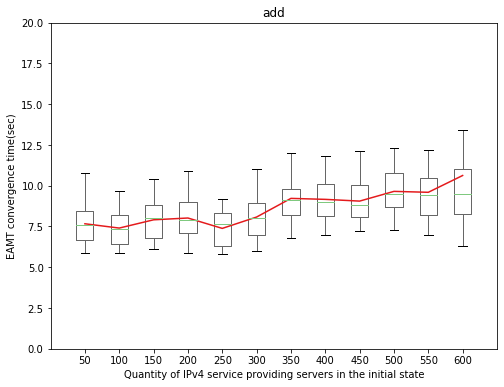
\includegraphics[width=12cm,pagebox=cropbox,clip]{img/eval2_result_add.png}
    \end{center}
    \caption{評価実験2:IPv4サービス提供サーバの追加を行った際のEAMT収束時間の比較}
    \label{fig:eval2_result_add}
\end{figure}


\begin{figure}[]
    \begin{center}
    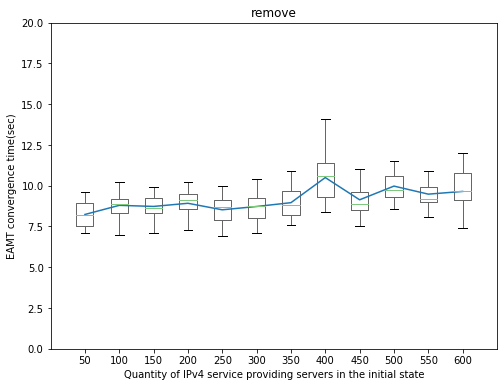
\includegraphics[width=12cm,pagebox=cropbox,clip]{img/eval2_result_remove.png}
    \end{center}
    \caption{評価実験2:IPv4サービス提供サーバの削除を行った際のEAMT収束時間の比較}
    \label{fig:eval2_result_remove}
\end{figure}



\newpage
\section{考察}
\label{evaluation:consideration}
本評価実験1の結果(\ref{evaluation:eval1:result})を通して本提案手法が各BRの一貫性の維持に有効であることが,本評価実験2の結果(\ref{evaluation:eval2:result})を通して本提案手法が変更追従性を十分に有していることがわかった.

しかしながらIPv4サービス提供サーバ数$x$が大きい場合においては,ルートリフレクタのパフォーマンスの悪化を読み取る事ができる

本評価実験環境においては,PoCで利用したルートリフレクタが適切に維持出来るBGPコネクション数の制限が表面化している.本問題に関しては以下のような取り組みが有効であると考えられる.
\begin{itemize}
    \item BGPパラメータの変更 \\
    本評価実験では,BGP KEEPALIVEメッセージージに利用する各種パラメータに関して,\ref{table:eval_bgp_timer}で指定したような値を採用している.KeepAlive送信間隔をより大きくすることで,より多くのコネクションを収容可能になることが想定される.
    \item ルートリフレクタトポロジーの見直しによる負荷軽減 \\
    本実験環境ではルートリフレクタ2ホスト(rr01,rr02)と全てのサーバ間でBGPコネクションを確立する一層のルートリフレクタトポロジーを採用しているが,第\label{proposal:network_rr}項で述べたような多層的なツリー型トポロジーを取り入れることで,ルートリフレクタ1ホストあたりが保持しなければならないコネクション数の軽減が期待できる.
\end{itemize}



%%% Local Variables:
%%% mode: japanese-latex
%%% TeX-master: "../thesis"
%%% End:

\chapter{結論}
\label{conclusion}

本章では,本研究のまとめと今後の課題を示す.

\section{本研究のまとめ}
本研究では,IPv6シングルスタックネットワークにおけるIPv4サービス提供手法として,ステートレスアドレス変換を利用した"SIIT-DC"と呼ばれるネットワークデザインに注目し,冗長性や変更追従性の問題を解決するために,考えられるアプローチを比較した上で,動的経路制御プロトコルであるBGPを利用したアドレス変換テーブルの広告・制御プロトコルを設計した.

本手法を評価するために,OSS及び自作のを利用したPoCを実装し,30台のBR,2台のルートリフレクタ,最大600台のサーバからなる評価用ネットワークにて2つのシナリオからなる評価実験を行った.
本評価実験の結果,本手法がSIIT-DCの冗長性と変更追従性を改善するフィジビリティを十分に有することが明らかになった.

\section{よりスケーラブルなBGPコネクショントポロジについての検討}
本評価実験を通して,ルートリフレクタが保有するべきBGPコネクションの数が大きくなることが,IPv4サービス提供サーバの収容可能台数と変更追従性に影響を及ぼすことがわかっている.

これはBGPコネクショントポロジを階層的なものにすることで,よりスケーラブルに本提案手法を運用することが可能である.
本節では2層のツリー型トポロジで接続されたルートリフレクタ群のスケーラビリティを定式化し,本提案手法の潜在的なスケーラビリティを明らかにする.

\subsection{2層のツリー型コネクショントポロジ}
\label{conclusion:tree:2layer}

ルートリフレクタが収容可能なサーバ台数を拡大するBGPコネクション設計に,ツリー型トポロジによるルートリフレクタの多層化の活用を考案した.
本研究において,ルートリフレクタの多層化とは,ルートリフレクタ間でツリートポロジ型のコネクションを確立させるようにルートリフレクタを配置する手法と定義する.

2層のツリー型トポロジで接続されたSIIT-DCの各ノードの関係図\ref{fig:2layer_bgp_topology}に示す.BRとコネクションを接続するルートリフレクタを第一層,サーバとコネクションを接続するルートリフレクタを第二層とする.

このツリー型トポロジではIPv4サービス提供サーバ・ルートリフレクタ・BR間の冗長コネクション数を2として設計しており,本トポロジにおいて,IPv4サービス提供サーバ及び各BRが確立するBGPコネクションは2となる.

\begin{figure}[h]
    \begin{center}
    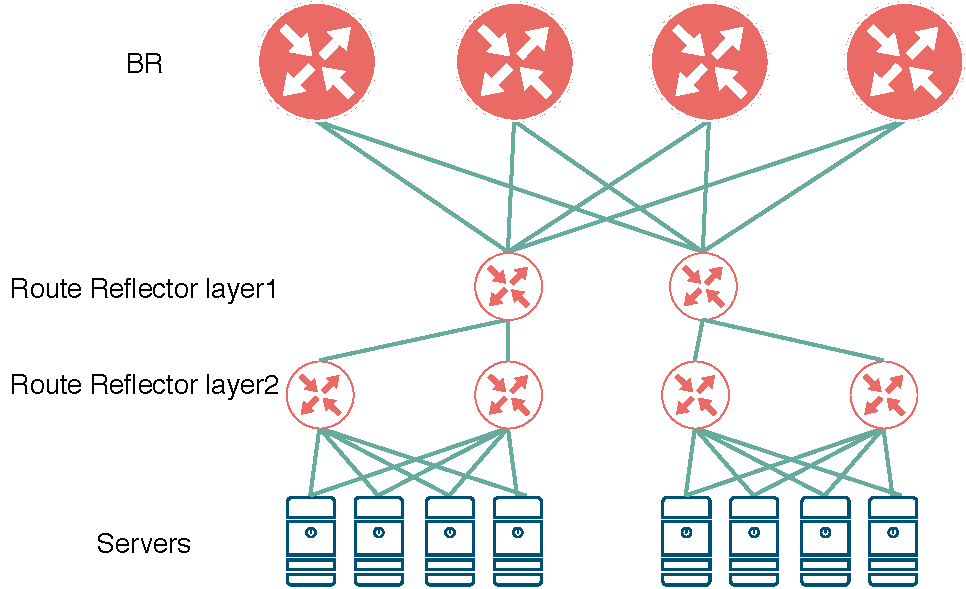
\includegraphics[width=12cm,pagebox=cropbox,clip]{img/2layer_bgp_topology_more_scale.pdf}
    \end{center}
    \caption{2層のBGPコネクショントポロジ}
    \label{fig:2layer_bgp_topology}
\end{figure}


また,本トポロジを採用したIDCネットワークにおける収容可能なサーバ数$S$は式\ref{eq:2layer_max_connection}のように示すことが出来る.この時,第一層のルートリフレクタの台数を2,BRのホスト数を$N$,第二層のルートリフレクタの台数を$L$,1台のルートリフレクタが収容可能なBGPピアの最大の数を$C_r$とする.


\begin{equation}
    S = \frac{L(C_r - N)}{2} \quad (L \leq C_r - N)
    \label{eq:2layer_max_connection}
\end{equation}


本研究において行った評価実験環境と同様に,1台のルートリフレクタが収容可能なBGPピア数$C_r$が630,BRの台数$N$が30である場合,本トポロジの最大収容可能サーバ数$S$は180000となる.

このようにBGPコネクショントポロジを多層化することで,BR及びIPv4サービス提供サーバが確立すべきコネクション数を増やすことなく,本提案手法のスケーラビリティをより高める事が可能になることがわかる.
同時に,本提案手法は数万台規模のサーバを抱える実際の商用ネットワークにおいても,本提案手法は高いスケーラビリティを有するモデルであると評価することが出来る.



% \subsection{EAMの集約}
% 本提案手法では,IPv4サービス提供サーバ自身がIPv4サービスアドレスを広告することを前提とした設計を行った.
% IPv4サービスアドレスを有するサーバ以外がEAMを複数集約して代理に広告するというユースケースを想定すると,BGPが利用するアドレスファミリの拡張仕様の設計が必要になると言える.


%%% Local Variables:
%%% mode: japanese-latex
%%% TeX-master: "../thesis"
%%% End:

%\appendix
\chapter{付録だよ}


\section{付録内容だよ}

書くよ

\chapter*{謝辞}
\addcontentsline{toc}{chapter}{謝辞}
\label{thanks}

% 先生に感謝
本論文の執筆にあたり,ご指導賜りました慶應義塾大学環境情報学部教授 村井純博士,環境情報学部教授 楠本博之博士,同学部教授 中村修博士,同学部教授 Rodny D.Van Meter 博士,同学部准教授 植原啓介博士,環境情報学部教授 三次仁博士,環境情報学部教授 中澤仁博士,同研究科特任教授 鈴木茂哉博士,政策・メディア研究科特任准教授 佐藤雅明博士,同研究科特任助教 工藤紀篤博士,同研究科特任講師 松谷健史博士に感謝致します.

特に,研究・運用・進路・私生活の多面において専らのご指導を下さいました中村修博士,植原啓介博士,佐藤雅明博士,近藤賢郎氏に重ねて深謝致します.運用ばかりで研究に手がつけられていなかった私を見捨てず,最後まで根気よくご指導頂いたこと,ただただ深謝の限りです.


% デルタメンに感謝
また,村井研究室での研究・運用・日常生活を共にした優秀な学生の皆様に感謝致します.特に,先輩として私の研究・運用活動に対する取り組み方をご指南頂きました,近藤賢郎氏,鈴木恒平氏,加藤桂子氏,阿部涼介氏,小林茉莉子氏,澤井優作氏,早川侑太郎氏,そしてrgroot・ORFNOCコアメンバーとして私の無謀な挑戦にご協力頂きました政策・メディア研究科 Korry Luke氏,総合政策学部 深川祐太氏,環境情報学部 栗原祐二氏,鈴木雄祐氏,平野孝徳氏,最後に修士・卒業論文で苦楽を共にした,政策・メディア研究科 亀井大向氏,草間好輝氏,今野嶺氏,環境情報学部 城一統氏に厚く御礼申し上げます.諸氏と過ごした「戦いの日々」を人生の糧として,今後より一層邁進致します.

% LINE株式会社に感謝
加えて,商用環境の何たるかを若輩物の私にご教示いただきましたLINE 株式会社 ネットワーク室 サービスネットワークチームの皆さま,特に同ネットワーク室長 白田篤志氏に感謝致します.約半年間の商用ネットワークのオペレーション経験は,本研究への取り組みの大きな糧となりました.重ね重ね御礼申し上げます.

% ナナヲアカリ・竜泉寺の湯に感謝
日本社会を支える皆さまに感謝致します.特に,執筆期間中の生活を物量面で支えてくれたセブンイレブン藤沢慶応大学前の皆さま,作業用BGMとして私の耳を癒やしてくれたナナヲアカリ氏,貴重な執筆場所として私を支えてくれた竜泉寺の湯湘南茅ヶ崎店の皆さまに深く感謝致します.



% 家族・さゆに感謝
最後に,生活, 精神両面で多大なる応援をして下さった家族そして須田小百合氏に厚くお礼申し上げます.特に須田小百合氏の存在が私の心身両面の支えとなりました.本当にありがとう御座いました.今後とも宜しくお願い致します.

以上を以って本論文の謝辞とさせていただきます.私を支えて下さった全ての方に重ねて感謝申し上げます.



%%% Local Variables:
%%% mode: japanese-latex
%%% TeX-master: "../yummy_bthesis"
%%% End:


\renewcommand{\thechapter}{\Alph{chapter}}
\setcounter{chapter}{0}
\vspace{-5mm}


\bibliographystyle{unsrt}\pagestyle{plain}
\bibliography{./bib/cites}\pagestyle{plain}
\thispagestyle{plain}%bibtex


\end{document}

%%% Local Variables:
%%% mode: japanese-latex
%%% TeX-master: t
%%% End:
